% ===========================================================================
\section{Results}
\label{sec:precise-alignment-results}
% ===========================================================================

This section reports quantitative registration results for both the LiDAR and stereo precise-alignment pipelines across nine experimental conditions conducted in the indoor laboratory environment described in \cref{subsubsec:pa-test-environment}. The nine conditions span a $3 \times 3$ factorial design of sensor-to-vine distance ($d \in \{40, 60, 80\}$\,cm) and approach angle ($\alpha \in \{-15^{\circ}, 0^{\circ}, +15^{\circ}\}$). Each LiDAR trial generates 35 perturbation hypotheses, yielding 315 hypothesis-level results in total; the stereo pipeline executes a single ICP run per trial. \Cref{tab:pa-results-condition-map} defines the mapping between experimental conditions and data identifiers.

% ---------------------------------------------------------------------------
\subsection{Trial Conditions and Mapping}
\label{subsec:pa-results-condition-map}
% ---------------------------------------------------------------------------

\begin{table}[htbp]
  \centering
  \caption{Experimental condition mapping. Each condition specifies the sensor-to-vine distance $d$ (cm) and approach angle $\alpha$ (degrees).}
  \label{tab:pa-results-condition-map}
  \begin{tabular}{@{} l r r @{}}
    \toprule
    \textbf{Condition} & \boldmath$d$ \textbf{(cm)} & \boldmath$\alpha$ \textbf{(°)} \\
    \midrule
    D40A$-$15 &  40 & $-$15 \\
    D40A0     &  40 &     0 \\
    D40A$+$15 &  40 & $+$15 \\
    D60A$-$15 &  60 & $-$15 \\
    D60A0     &  60 &     0 \\
    D60A$+$15 &  60 & $+$15 \\
    D80A$-$15 &  80 & $-$15 \\
    D80A0     &  80 &     0 \\
    D80A$+$15 &  80 & $+$15 \\
    \bottomrule
  \end{tabular}
\end{table}

% ---------------------------------------------------------------------------
\subsection{LiDAR Registration Performance}
\label{subsec:pa-results-lidar-summary}
% ---------------------------------------------------------------------------

\Cref{tab:pa-results-lidar-per-condition} summarises the LiDAR registration outcome for each condition. For each trial the table reports the number of points in the preprocessed source cloud, the number and proportion of the 35 hypotheses that exceeded the fitness acceptance threshold ($F \geq 0.8$), and the median and interquartile range (IQR) of the fitness score and inlier RMSE across accepted hypotheses.

\begin{table}[htbp]
  \centering
  \small
  \setlength{\tabcolsep}{4pt}
  \caption{Per-condition LiDAR registration summary. Median and IQR statistics are computed over accepted hypotheses only ($F \geq 0.8$). All inlier RMSE values are in millimetres.}
  \label{tab:pa-results-lidar-per-condition}
  \begin{tabular}{@{} l r r r r r r r @{}}
    \toprule
    \textbf{Condition} &
    \textbf{Proc.\ pts} &
    \boldmath$n_\text{acc}$\textbf{/35} &
    \textbf{\%} &
    \boldmath$\tilde{F}$ &
    \textbf{IQR(}\boldmath$F$\textbf{)} &
    \boldmath$\tilde{\varepsilon}$ \textbf{(mm)} &
    \textbf{IQR(}\boldmath$\varepsilon$\textbf{) (mm)} \\
    \midrule
    D40A$-$15 &  97\,358 & 35/35 & 100 & 0.8939 & 0.0079 & 32.31 & 2.37 \\
    D40A0     & 112\,312 & 34/35 &  97 & 0.9107 & 0.0000 & 35.22 & 0.27 \\
    D40A$+$15 & 111\,880 & 35/35 & 100 & 0.9042 & 0.0000 & 34.85 & 0.59 \\
    D60A$-$15 & 116\,892 & 35/35 & 100 & 0.9205 & 0.0001 & 34.94 & 0.10 \\
    D60A0     & 108\,707 & 35/35 & 100 & 0.9174 & 0.0000 & 33.25 & 0.00 \\
    D60A$+$15 & 111\,880 & 35/35 & 100 & 0.9042 & 0.0000 & 34.84 & 0.58 \\
    D80A$-$15 & 116\,750 & 35/35 & 100 & 0.9141 & 0.0001 & 23.38 & 0.02 \\
    D80A0     & 121\,350 & 32/35 &  91 & 0.9277 & 0.0000 & 24.41 & 0.00 \\
    D80A$+$15 & 133\,017 & 35/35 & 100 & 0.9160 & 0.0000 & 23.77 & 0.00 \\
    \midrule
    \textbf{Aggregate} & --- & 311/315 & 98.7 & 0.9141 & 0.0133 & 33.25 & 10.47 \\
    \bottomrule
  \end{tabular}
\end{table}

All nine conditions achieved full or near-full hypothesis acceptance ($\geq 91\%$). Of the 315 hypotheses evaluated, 311 were accepted (98.7\%). The lowest per-condition acceptance rate was D80A0 at 91\% (32/35); the remaining eight conditions achieved 97--100\%.

% ---------------------------------------------------------------------------
\subsection{Per-Perturbation-Group Results}
\label{subsec:pa-results-perturbation-groups}
% ---------------------------------------------------------------------------

The 35 hypotheses generated per trial are organised into five perturbation groups. Statistics in \cref{tab:pa-results-groups} are aggregated across all nine conditions (315 hypotheses total); metrics are computed over accepted hypotheses only.

\begin{itemize}
  \item \emph{Orig} (1 per trial): the nominal, unperturbed initial pose.
  \item \emph{Group~A} (6 per trial): axis-aligned translation perturbations ($\pm x$, $\pm y$, $\pm z$).
  \item \emph{Group~B} (4 per trial): cardinal-direction translations (N, E, S, W).
  \item \emph{Group~C} (12 per trial): compound perturbations combining diagonal translations with yaw rotations.
  \item \emph{Group~E} (12 per trial): rotation-only perturbations sweeping yaw, pitch, and roll.
\end{itemize}

\begin{table}[htbp]
  \centering
  \small
  \setlength{\tabcolsep}{4pt}
  \caption{Per-perturbation-group registration results, aggregated across all nine conditions (315 hypotheses total). Statistics computed over accepted hypotheses only.}
  \label{tab:pa-results-groups}
  \begin{tabular}{@{} l r r r r r r @{}}
    \toprule
    \textbf{Group} &
    \boldmath$n_\text{acc}$\textbf{/}\boldmath$n_\text{hyp}$ &
    \textbf{\%} &
    \boldmath$\tilde{F}$ &
    \textbf{IQR(}\boldmath$F$\textbf{)} &
    \boldmath$\tilde{\varepsilon}$ \textbf{(mm)} &
    \textbf{IQR(}\boldmath$\varepsilon$\textbf{) (mm)} \\
    \midrule
    Orig   &   9/9   & 100 & 0.9142 & 0.0133 & 34.28 & 10.25 \\
    A      &  54/54  & 100 & 0.9141 & 0.0133 & 33.25 & 10.47 \\
    B      &  36/36  & 100 & 0.9141 & 0.0133 & 33.77 & 10.44 \\
    C      & 105/108 &  97 & 0.9107 & 0.0133 & 34.84 & 10.62 \\
    E      & 107/108 &  99 & 0.9141 & 0.0133 & 33.25 & 10.47 \\
    \midrule
    \textbf{All} & 311/315 & 99 & 0.9141 & 0.0133 & 33.25 & 10.47 \\
    \bottomrule
  \end{tabular}
\end{table}

Acceptance rates range from 97\% (Group~C) to 100\% (Orig, A, B). Median fitness and RMSE are consistent across all groups.

% ---------------------------------------------------------------------------
\subsection{LiDAR: Distance and Angle Effects}
\label{subsec:pa-results-lidar-distance-angle}
% ---------------------------------------------------------------------------

\Cref{tab:pa-results-lidar-by-distance,tab:pa-results-lidar-by-angle} present registration outcomes grouped by sensor-to-vine distance and approach angle, respectively.

\begin{table}[htbp]
  \centering
  \caption{LiDAR registration results grouped by sensor-to-vine distance. Best-hypothesis fitness and RMSE are reported (median across conditions within each distance group). All RMSE values in millimetres.}
  \label{tab:pa-results-lidar-by-distance}
  \begin{tabular}{@{} l r r r r r @{}}
    \toprule
    \textbf{Distance} &
    \textbf{Conditions} &
    \boldmath$n_\text{acc}$\textbf{/}\boldmath$n_\text{total}$ &
    \textbf{\%} &
    \textbf{Med.\ best} \boldmath$F$ &
    \textbf{Med.\ best} \boldmath$\varepsilon$ \textbf{(mm)} \\
    \midrule
    D40 (40\,cm)  & 3 & 104/105 &  99 & 0.9042 & 34.66 \\
    D60 (60\,cm)  & 3 & 105/105 & 100 & 0.9174 & 34.29 \\
    D80 (80\,cm)  & 3 & 102/105 &  97 & 0.9160 & 23.77 \\
    \bottomrule
  \end{tabular}
\end{table}

\begin{table}[htbp]
  \centering
  \caption{LiDAR registration results grouped by approach angle. All RMSE values in millimetres.}
  \label{tab:pa-results-lidar-by-angle}
  \begin{tabular}{@{} l r r r r r @{}}
    \toprule
    \textbf{Angle} &
    \textbf{Conditions} &
    \boldmath$n_\text{acc}$\textbf{/}\boldmath$n_\text{total}$ &
    \textbf{\%} &
    \textbf{Med.\ best} \boldmath$F$ &
    \textbf{Med.\ best} \boldmath$\varepsilon$ \textbf{(mm)} \\
    \midrule
    A$-$15 ($-15^{\circ}$) & 3 & 105/105 & 100 & 0.9143 & 34.66 \\
    A0 ($0^{\circ}$)       & 3 & 101/105 &  96 & 0.9174 & 33.25 \\
    A$+$15 ($+15^{\circ}$) & 3 & 105/105 & 100 & 0.9042 & 34.28 \\
    \bottomrule
  \end{tabular}
\end{table}

The D40, D60, and D80 distance groups all achieve acceptance rates above 97\%. The D80 group exhibits a lower median best RMSE (23.77\,mm) compared to D40 (34.66\,mm) and D60 (34.29\,mm). Across approach angles, acceptance rates are 100\% for both A$-$15 and A$+$15, and 96\% for A0.

% ---------------------------------------------------------------------------
\subsection{LiDAR: Recovered ICP Correction}
\label{subsec:pa-results-lidar-transformation}
% ---------------------------------------------------------------------------

\Cref{tab:pa-results-lidar-icp-correction} reports the positional displacement and rotation correction applied by the GICP solver for the best-selected hypothesis in each condition. The translational displacement $\lVert\Delta\mathbf{t}\rVert$ is the Euclidean distance between the initial and final sensor positions; component displacements ($\Delta x$, $\Delta y$, $\Delta z$) are in the local ENU frame. Rotations are ZYX Euler angles extracted from the correction matrix.

\begin{table}[htbp]
  \centering
  \small
  \setlength{\tabcolsep}{3pt}
  \caption{ICP correction for the best-selected hypothesis per condition. Translational displacement in millimetres; rotation corrections as ZYX Euler angles in degrees.}
  \label{tab:pa-results-lidar-icp-correction}
  \begin{tabular}{@{} l r r r r r r r @{}}
    \toprule
    \textbf{Condition} &
    \boldmath$\lVert\Delta\mathbf{t}\rVert$ \textbf{(mm)} &
    \boldmath$\Delta x$ \textbf{(mm)} &
    \boldmath$\Delta y$ \textbf{(mm)} &
    \boldmath$\Delta z$ \textbf{(mm)} &
    \boldmath$\Delta\psi$ \textbf{(°)} &
    \boldmath$\Delta\theta$ \textbf{(°)} &
    \boldmath$\Delta\phi$ \textbf{(°)} \\
    \midrule
    D40A$-$15 &  90.6 &    25.2 &    13.8 &    85.9 & $-$1.70 &    1.84 & $-$10.48 \\
    D40A0     & 143.8 &    17.2 &    39.8 &   137.1 &    0.13 &    3.46 &  $-$7.21 \\
    D40A$+$15 &  91.9 &    28.3 &    15.3 &    86.1 & $-$1.54 &    1.60 & $-$11.48 \\
    D60A$-$15 & 148.0 &    89.0 & $-$70.0 &    95.3 &    4.41 &    8.49 &  $-$5.24 \\
    D60A0     & 106.7 & $-$41.1 &    57.9 &    79.7 & $-$2.70 &    3.07 &  $-$4.03 \\
    D60A$+$15 &  92.0 &    27.7 &    16.9 &    86.0 & $-$1.54 &    1.59 & $-$11.45 \\
    D80A$-$15 & 165.3 & $-$120.6 & $-$2.3 &   113.1 &    2.04 &    5.35 &  $-$3.52 \\
    D80A0     & 136.3 & $-$37.0 &    85.5 &    99.4 & $-$2.95 & $-$0.36 &  $-$7.50 \\
    D80A$+$15 & 131.3 & $-$85.2 &    77.8 &    62.7 & $-$5.98 &    0.21 &  $-$5.42 \\
    \bottomrule
  \end{tabular}
\end{table}

For the nine converging conditions, the mean positional displacement is 122.9\,mm (max 165.3\,mm, D80A$-$15), confirming that ICP adjustments remain within the expected range of the initial pose estimate. The roll correction ($\Delta\phi$) is consistently negative, ranging from $-3.5^{\circ}$ to $-11.5^{\circ}$. Rotational corrections range from 0.13° to 11.48° in magnitude.

% ---------------------------------------------------------------------------
\subsection{LiDAR: Within-Trial Convergence}
\label{subsec:pa-results-lidar-convergence}
% ---------------------------------------------------------------------------

\Cref{tab:pa-results-lidar-sigma} reports the standard deviation ($\sigma$) of the recovered transformation components across accepted hypotheses within each condition.

\begin{table}[htbp]
  \centering
  \small
  \setlength{\tabcolsep}{3pt}
  \caption{Standard deviation of recovered final pose components across accepted hypotheses within each condition. Low values indicate that multiple initial perturbations converge to the same final alignment. Translation values in metres; rotation values in degrees.}
  \label{tab:pa-results-lidar-sigma}
  \begin{tabular}{@{} l r r r r r r r @{}}
    \toprule
    \textbf{Condition} &
    \boldmath$n_\text{acc}$ &
    \boldmath$\sigma_{t_x}$ &
    \boldmath$\sigma_{t_y}$ &
    \boldmath$\sigma_{t_z}$ &
    \boldmath$\sigma_{\psi}$ \textbf{(°)} &
    \boldmath$\sigma_{\theta}$ \textbf{(°)} &
    \boldmath$\sigma_{\phi}$ \textbf{(°)} \\
    \midrule
    D40A$-$15 & 35 & 0.002 & 0.010 & 0.025 & 1.09 & 2.28 & 4.06 \\
    D40A0     & 34 & 0.002 & 0.002 & 0.001 & 0.06 & 0.70 & 0.44 \\
    D40A$+$15 & 35 & 0.005 & 0.009 & 0.030 & 1.11 & 2.21 & 4.21 \\
    D60A$-$15 & 35 & 0.005 & 0.004 & 0.005 & 0.30 & 1.26 & 1.04 \\
    D60A0     & 35 & 0.134 & 0.078 & 0.014 & 0.26 & 1.18 & 0.46 \\
    D60A$+$15 & 35 & 0.004 & 0.009 & 0.026 & 1.03 & 1.99 & 3.80 \\
    D80A$-$15 & 35 & 0.069 & 0.001 & 0.091 & 0.50 & 1.54 & 6.71 \\
    D80A0     & 32 & 0.000 & 0.000 & 0.000 & 0.00 & 0.00 & 0.00 \\
    D80A$+$15 & 35 & 0.066 & 0.004 & 0.083 & 0.37 & 1.70 & 6.05 \\
    \bottomrule
  \end{tabular}
\end{table}

D80A0 achieves near-zero spread across all components ($\sigma < 0.1$\,mm, $< 0.01^{\circ}$), indicating convergence to a single pose. D60A0 exhibits an elevated $\sigma_{t_x}$ of 134\,mm. D80A$-$15 and D80A$+$15 show the largest roll variability ($\sigma_\phi > 6^{\circ}$). D40A$-$15 and D40A$+$15 exhibit moderate roll variability ($\sigma_\phi \approx 4^{\circ}$).

% ---------------------------------------------------------------------------
\subsection{LiDAR: Pipeline Timing}
\label{subsec:pa-results-lidar-timing}
% ---------------------------------------------------------------------------

\Cref{tab:pa-results-lidar-timing} reports wall-clock timing for each condition. The 25\,s scan accumulation interval preceding the pipeline is excluded, as accumulation for the next vine can be performed concurrently with pruning of the current vine.

\begin{table}[htbp]
  \centering
  \caption{Per-condition LiDAR pipeline timing. Preprocessing covers sensor data filtering to source cloud; ICP/trial is the mean per-hypothesis registration time; total covers preprocessing through pose publication across all 35 hypotheses.}
  \label{tab:pa-results-lidar-timing}
  \begin{tabular}{@{} l r r r @{}}
    \toprule
    \textbf{Condition} &
    \textbf{Preprocess (s)} &
    \textbf{ICP/trial (s)} &
    \textbf{Total (s)} \\
    \midrule
    D40A$-$15 & 0.61 & 0.89 & 42.8 \\
    D40A0     & 0.74 & 1.11 & 50.9 \\
    D40A$+$15 & 0.67 & 0.98 & 47.4 \\
    D60A$-$15 & 0.71 & 1.16 & 53.3 \\
    D60A0     & 0.65 & 0.89 & 43.0 \\
    D60A$+$15 & 0.66 & 0.96 & 46.2 \\
    D80A$-$15 & 0.72 & 0.84 & 41.5 \\
    D80A0     & 0.79 & 0.87 & 43.3 \\
    D80A$+$15 & 0.82 & 0.91 & 45.5 \\
    \midrule
    \textbf{Mean $\pm$ std} & $0.71 \pm 0.06$ & $0.96 \pm 0.10$ & $46.0 \pm 3.8$ \\
    \bottomrule
  \end{tabular}
\end{table}

For all nine conditions, preprocessing requires 0.61--0.82\,s, per-hypothesis ICP registration requires 0.84--1.16\,s, and total pipeline latency ranges from 41.5 to 53.3\,s with a mean of $46.0 \pm 3.8$\,s.

% ---------------------------------------------------------------------------
\subsection{LiDAR: Visual Alignment}
\label{subsec:pa-results-lidar-visual}
% ---------------------------------------------------------------------------

\Cref{fig:pa-lidar-heatmap} presents a heatmap of ICP fitness across all 315 hypotheses (9 conditions $\times$ 35 perturbations), providing an overview of registration success across the experimental matrix.

\begin{figure}[htbp]
  \centering
  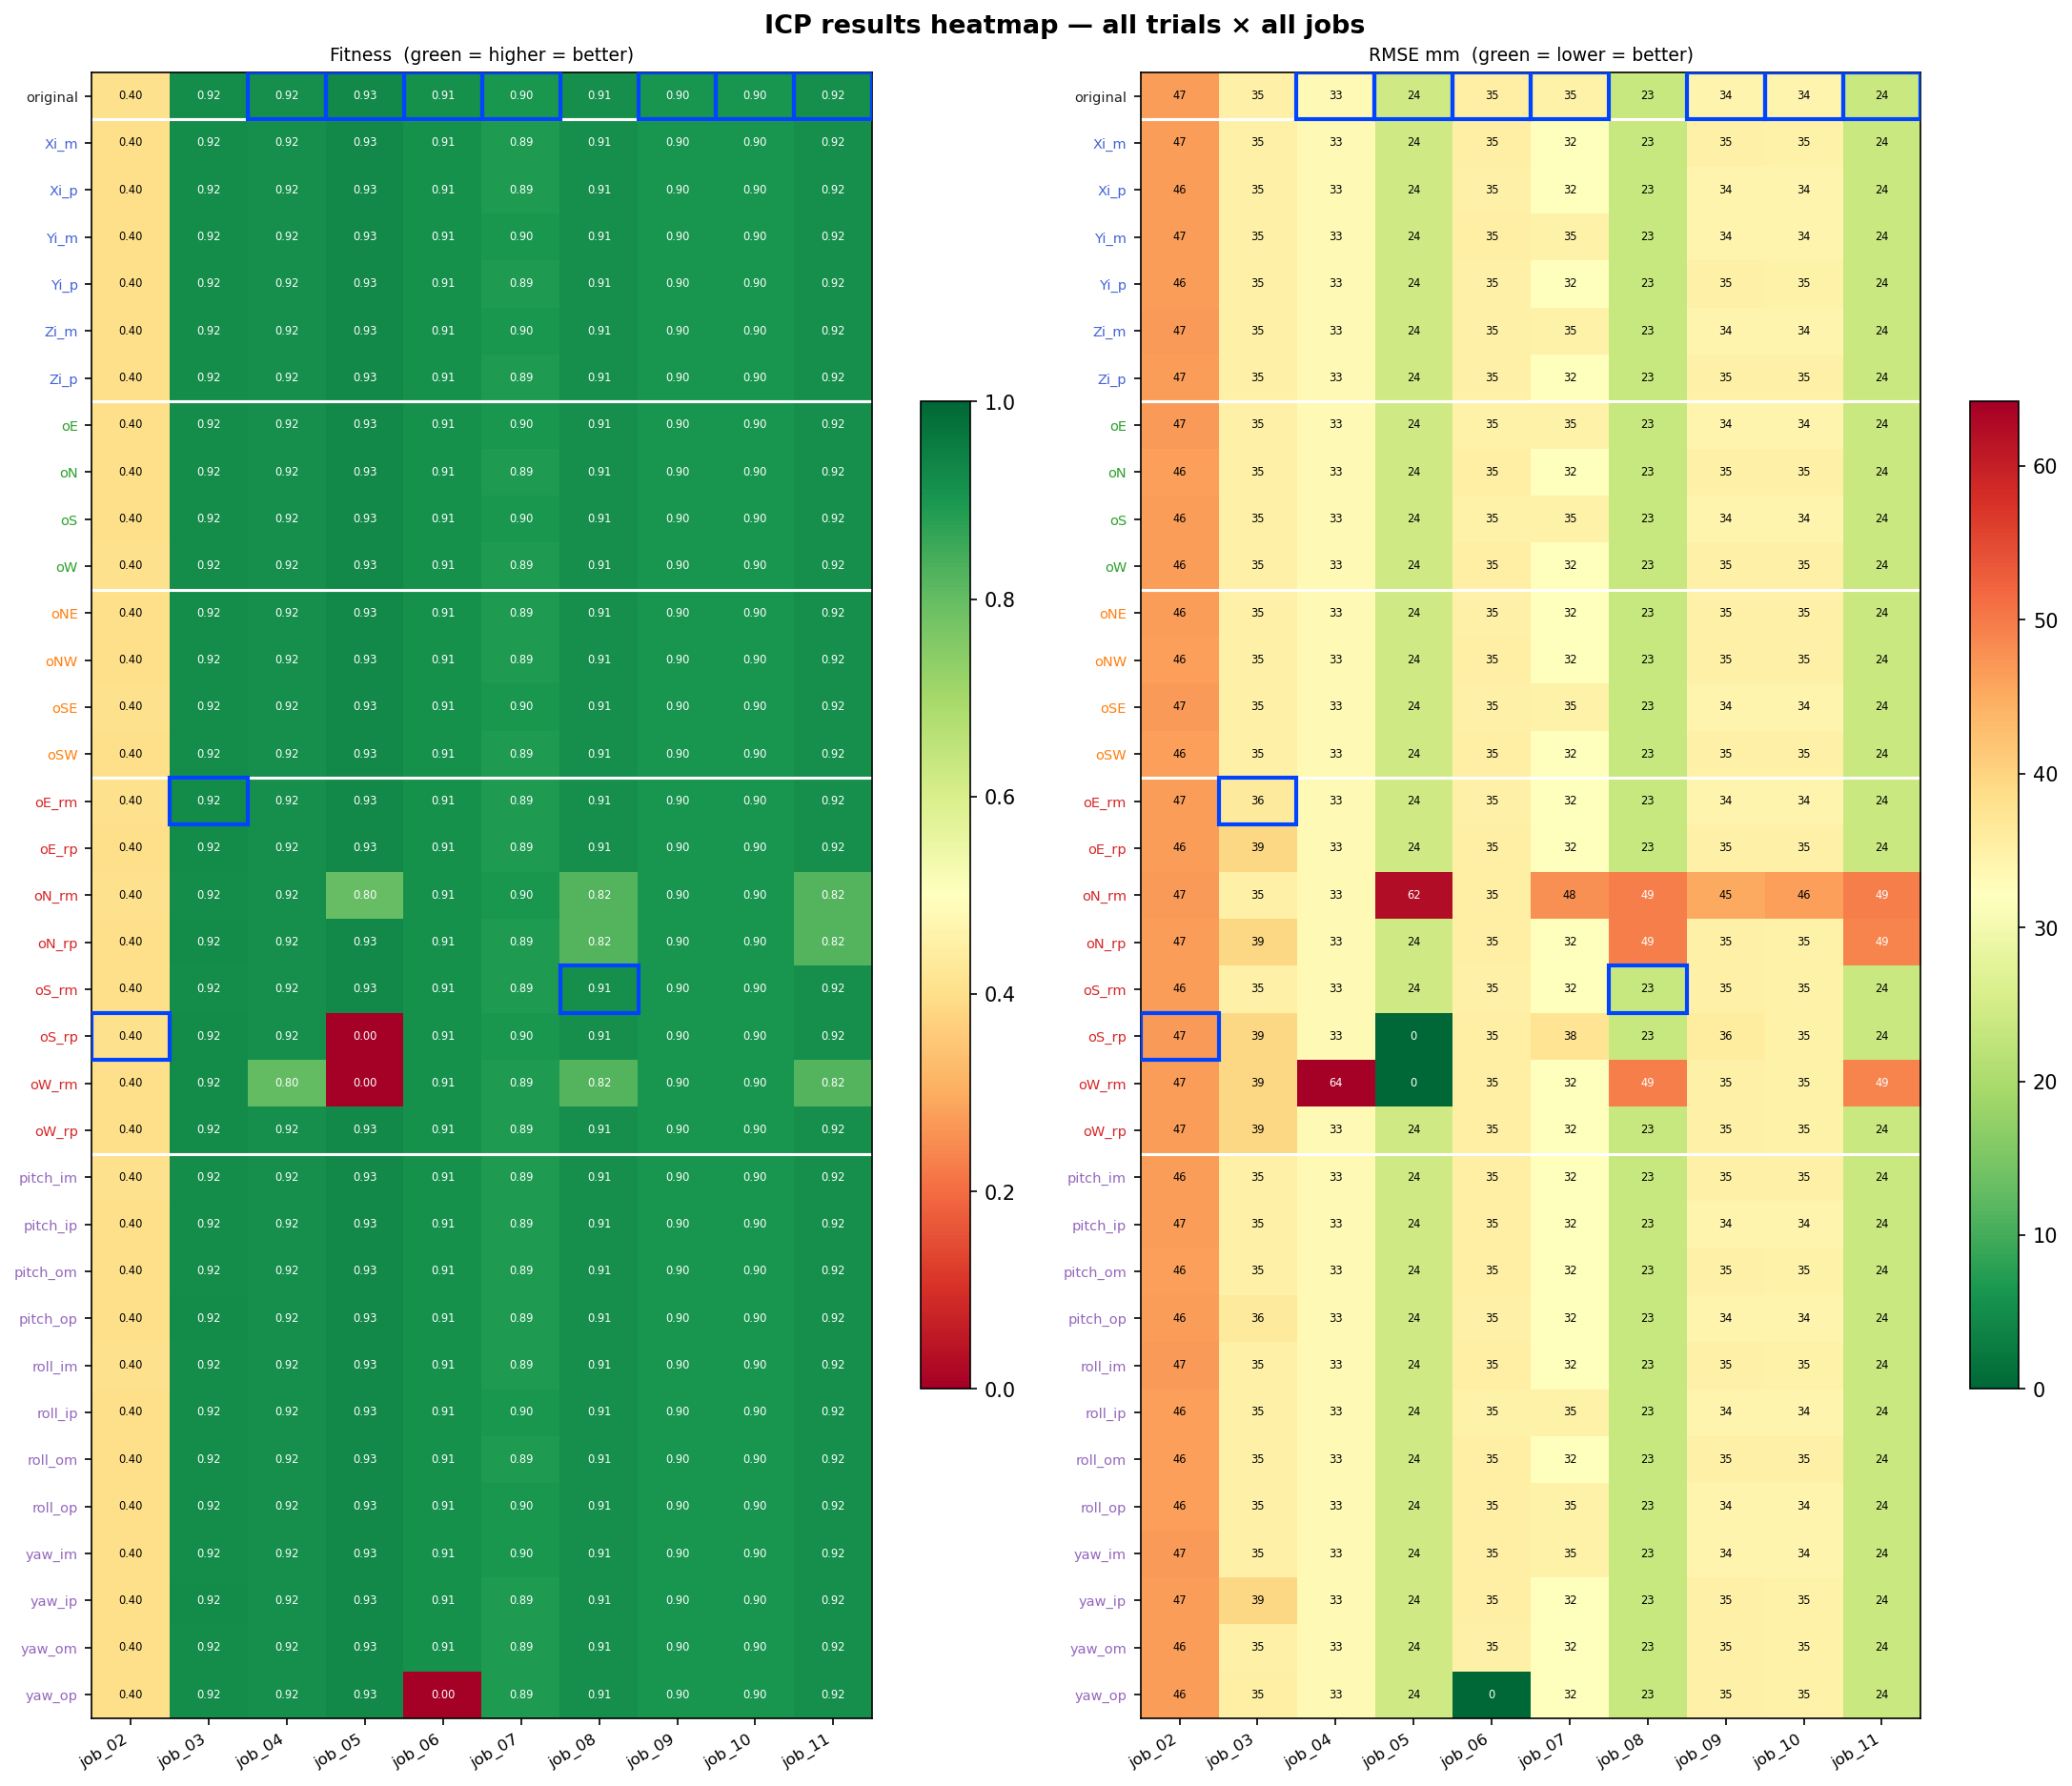
\includegraphics[width=\linewidth]{4-precise-alignment/4-results/figures/lidar_icp_heatmap}
  \caption{ICP fitness heatmap across all hypotheses. Each row corresponds to one condition (ordered by distance); each column to one perturbation hypothesis. Colour intensity indicates fitness score. The D110A0 row visible in this figure was excluded from analysis as it exceeded the stereo pipeline's depth clipping threshold.}
  \label{fig:pa-lidar-heatmap}
\end{figure}

\Cref{fig:pa-lidar-alignment-examples} presents representative alignment visualisations for selected conditions spanning the distance range.

\begin{figure}[htbp]
  \centering
  \begin{subfigure}[b]{0.48\linewidth}
    \centering
    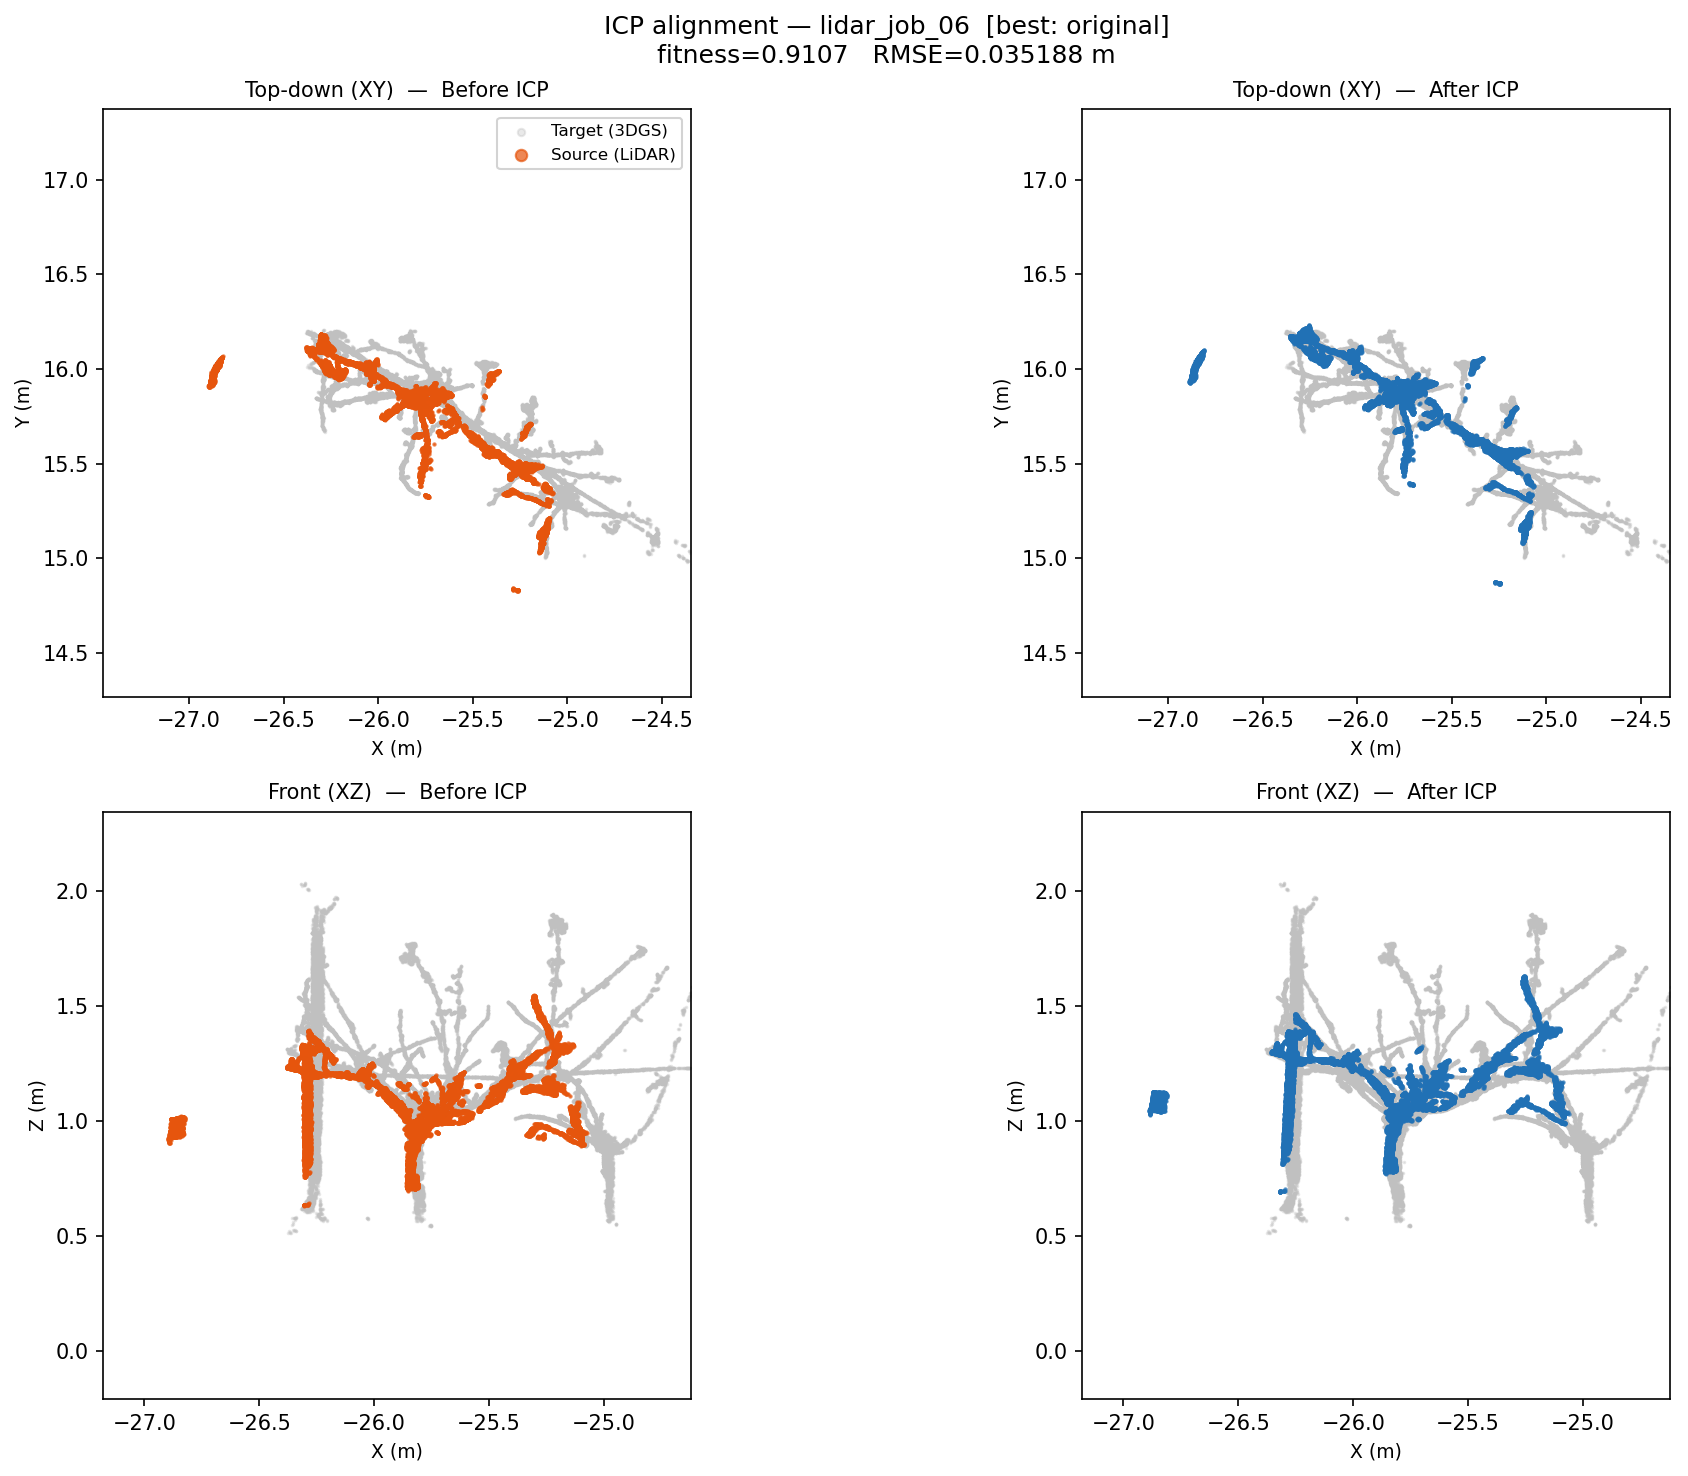
\includegraphics[width=\linewidth]{4-precise-alignment/4-results/figures/lidar_D40A0_alignment}
    \caption{D40A0 (40\,cm, $0^{\circ}$)}
    \label{fig:pa-lidar-align-D40A0}
  \end{subfigure}
  \hfill
  \begin{subfigure}[b]{0.48\linewidth}
    \centering
    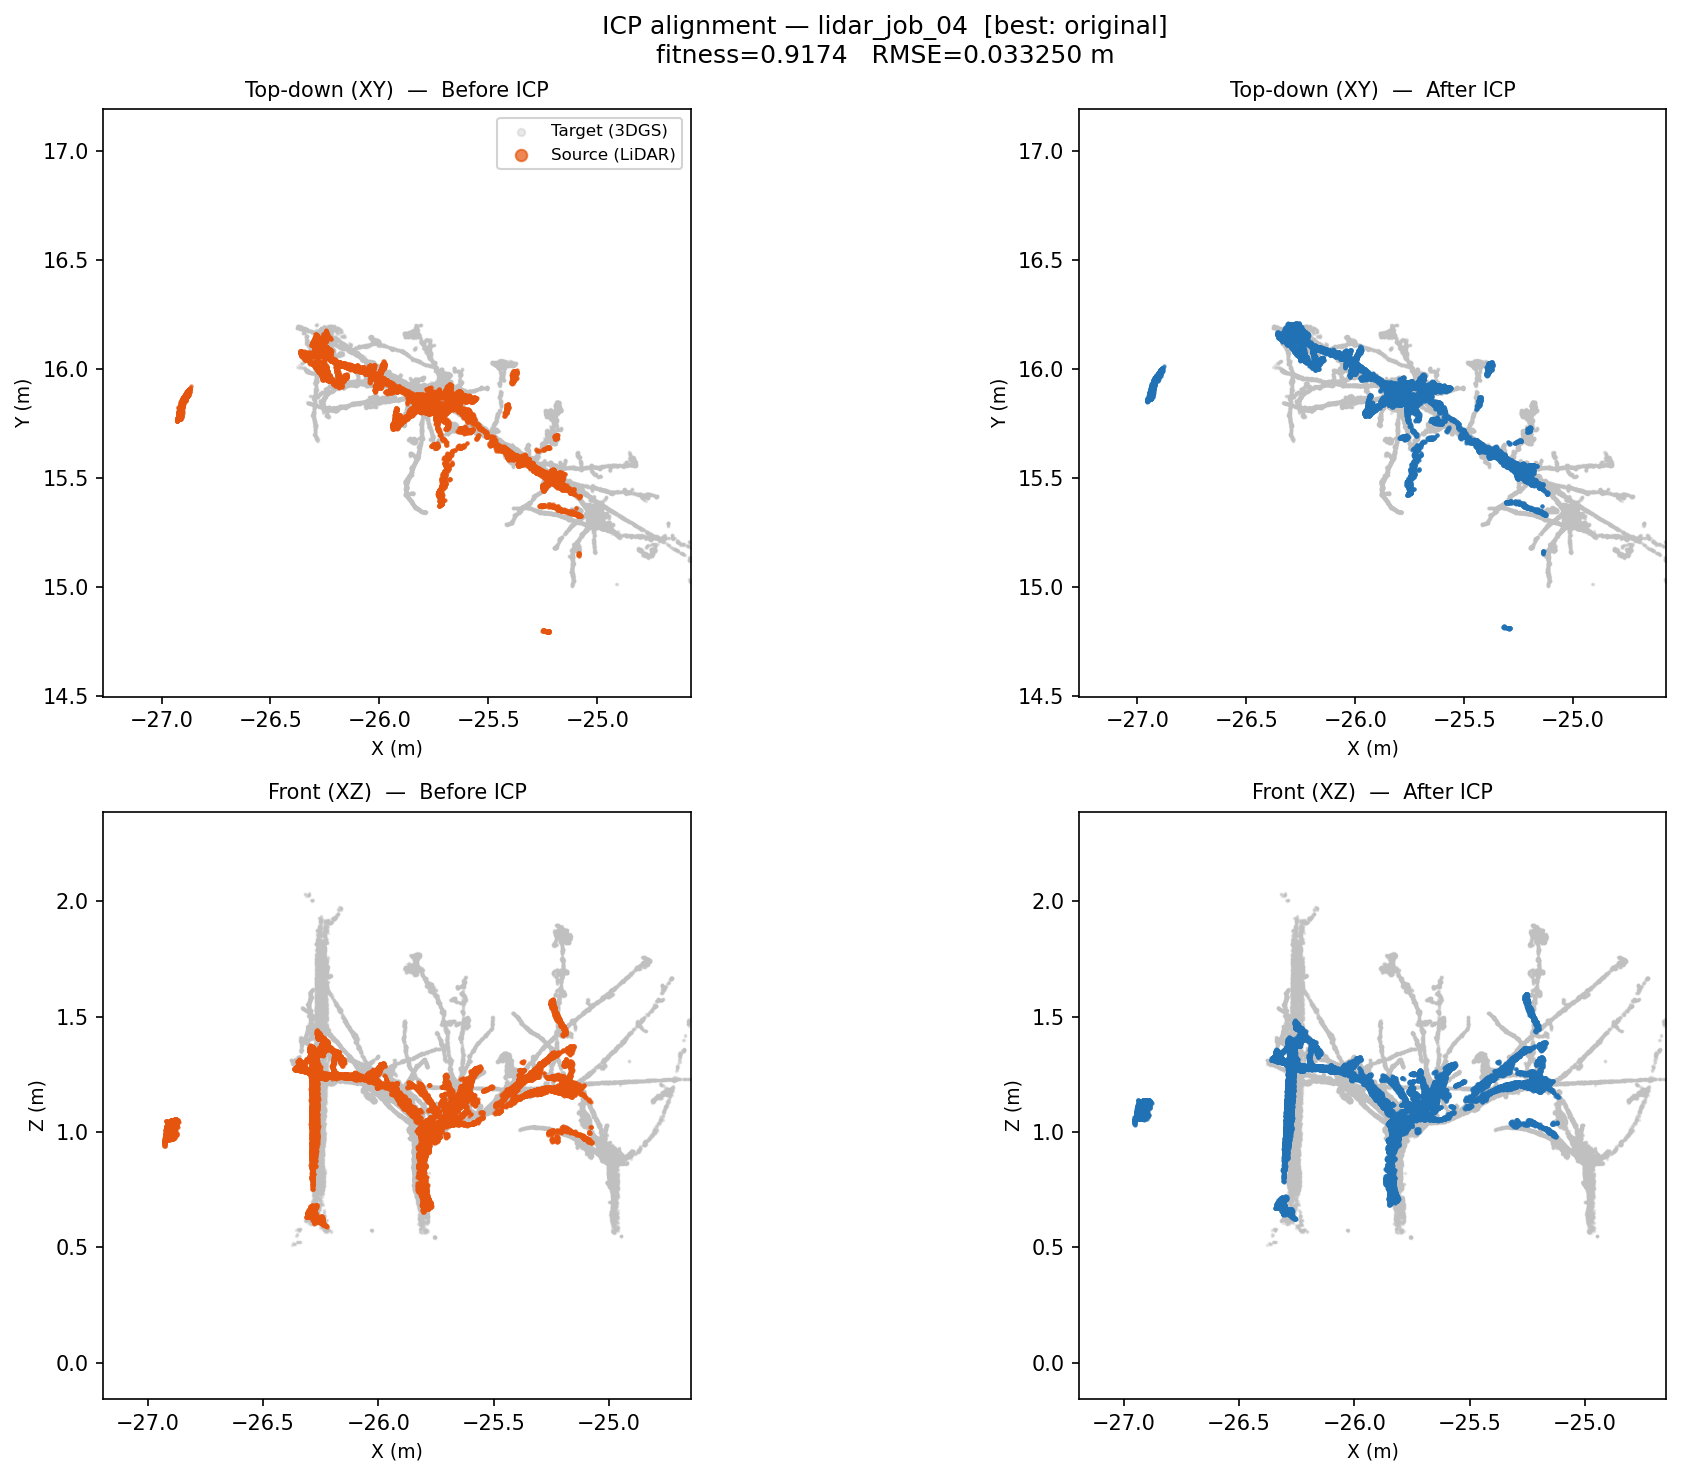
\includegraphics[width=\linewidth]{4-precise-alignment/4-results/figures/lidar_D60A0_alignment}
    \caption{D60A0 (60\,cm, $0^{\circ}$)}
    \label{fig:pa-lidar-align-D60A0}
  \end{subfigure}

  \vspace{0.5em}

  \begin{subfigure}[b]{0.48\linewidth}
    \centering
    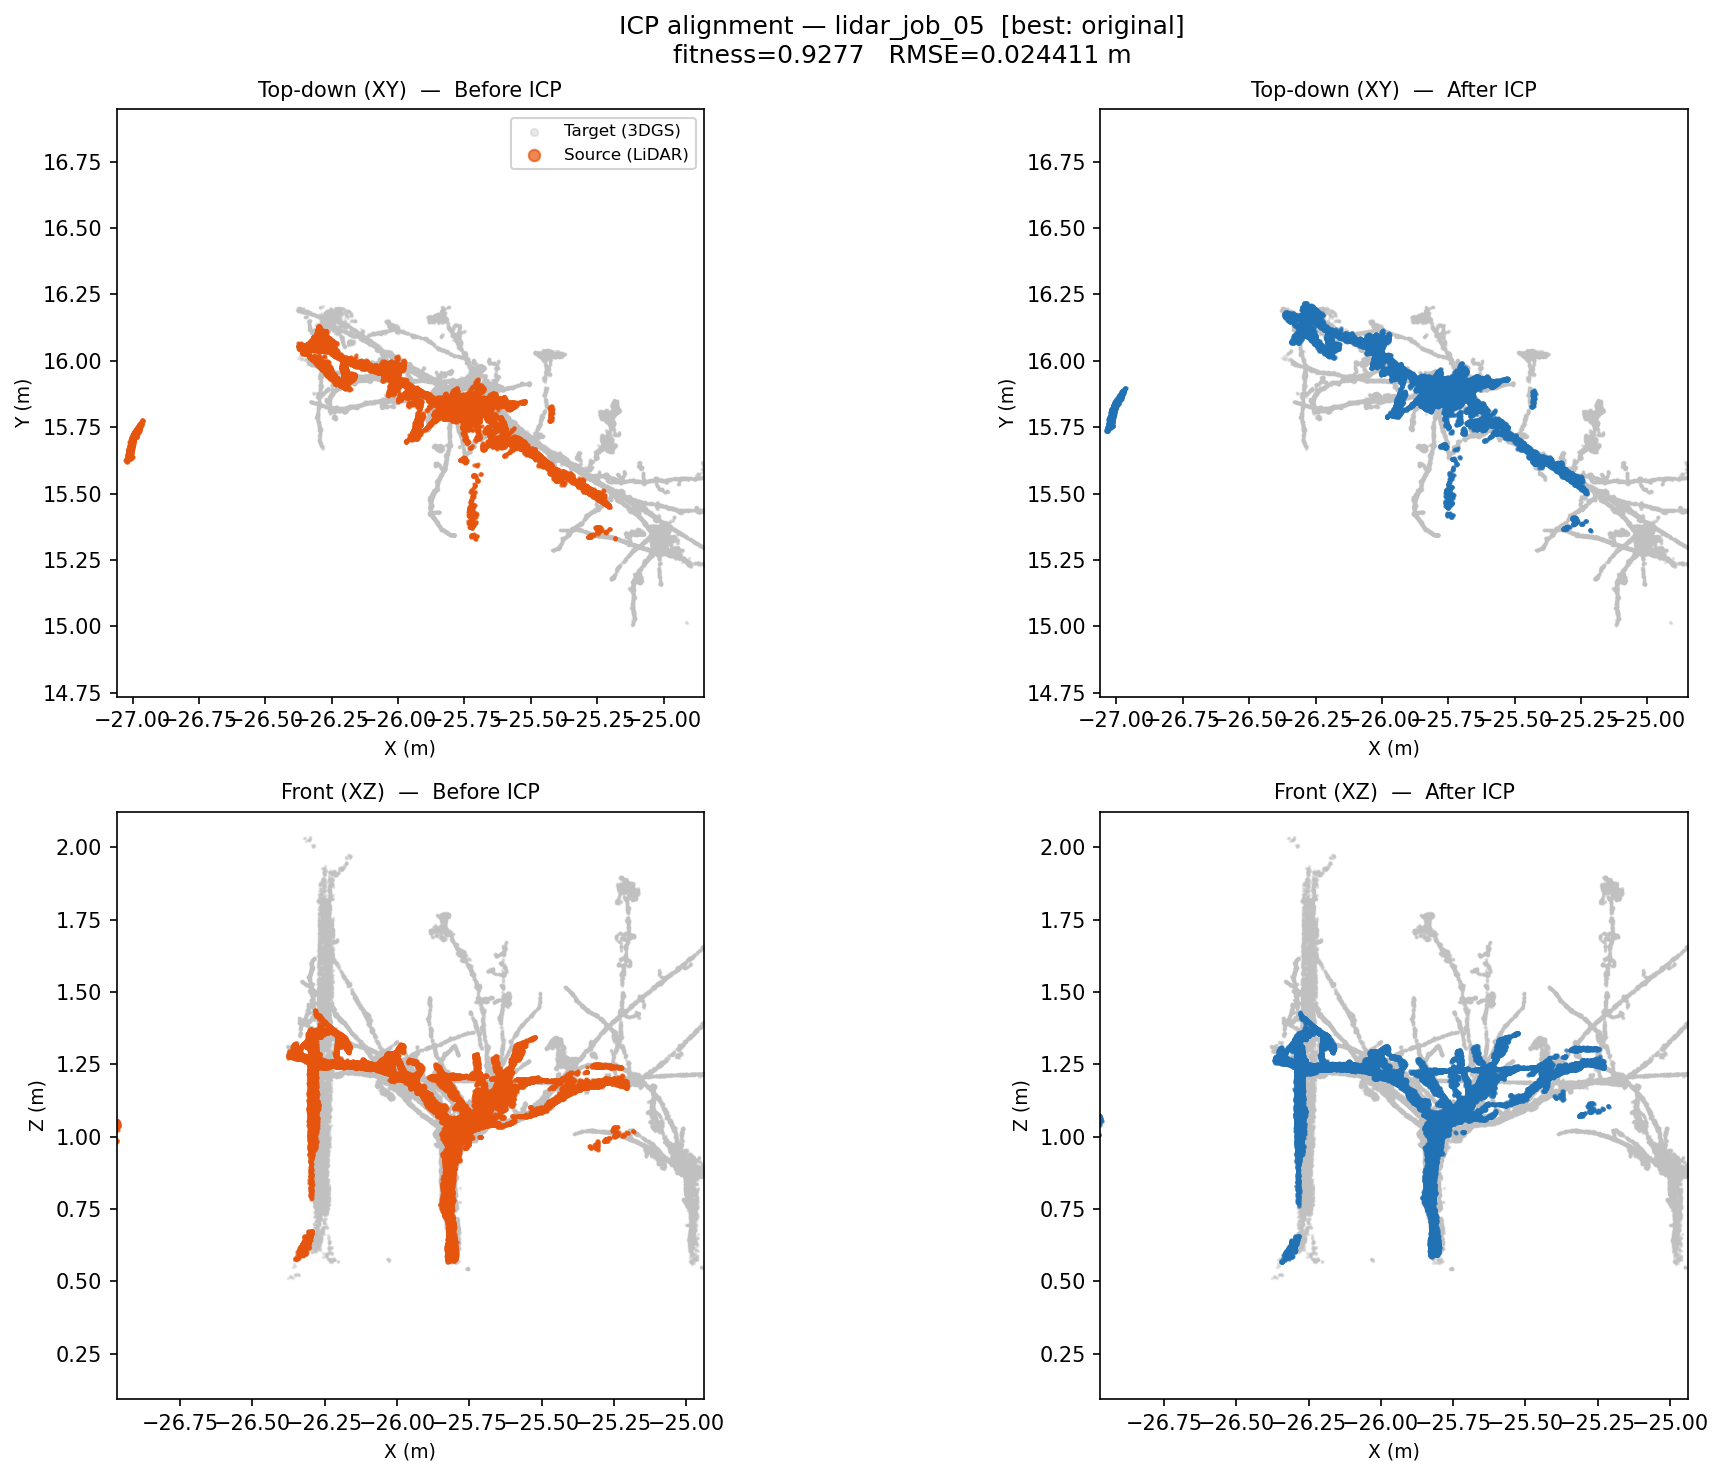
\includegraphics[width=\linewidth]{4-precise-alignment/4-results/figures/lidar_D80A0_alignment}
    \caption{D80A0 (80\,cm, $0^{\circ}$)}
    \label{fig:pa-lidar-align-D80A0}
  \end{subfigure}
  \caption{LiDAR alignment visualisations for the best-selected hypothesis at each $0^{\circ}$ approach angle condition. Source cloud (coloured) overlaid on the 3DGS reference target (grey).}
  \label{fig:pa-lidar-alignment-examples}
\end{figure}

\Cref{fig:pa-lidar-batch-summary} presents the batch summary comparing best-trial registration metrics across all nine conditions.

\begin{figure}[htbp]
  \centering
  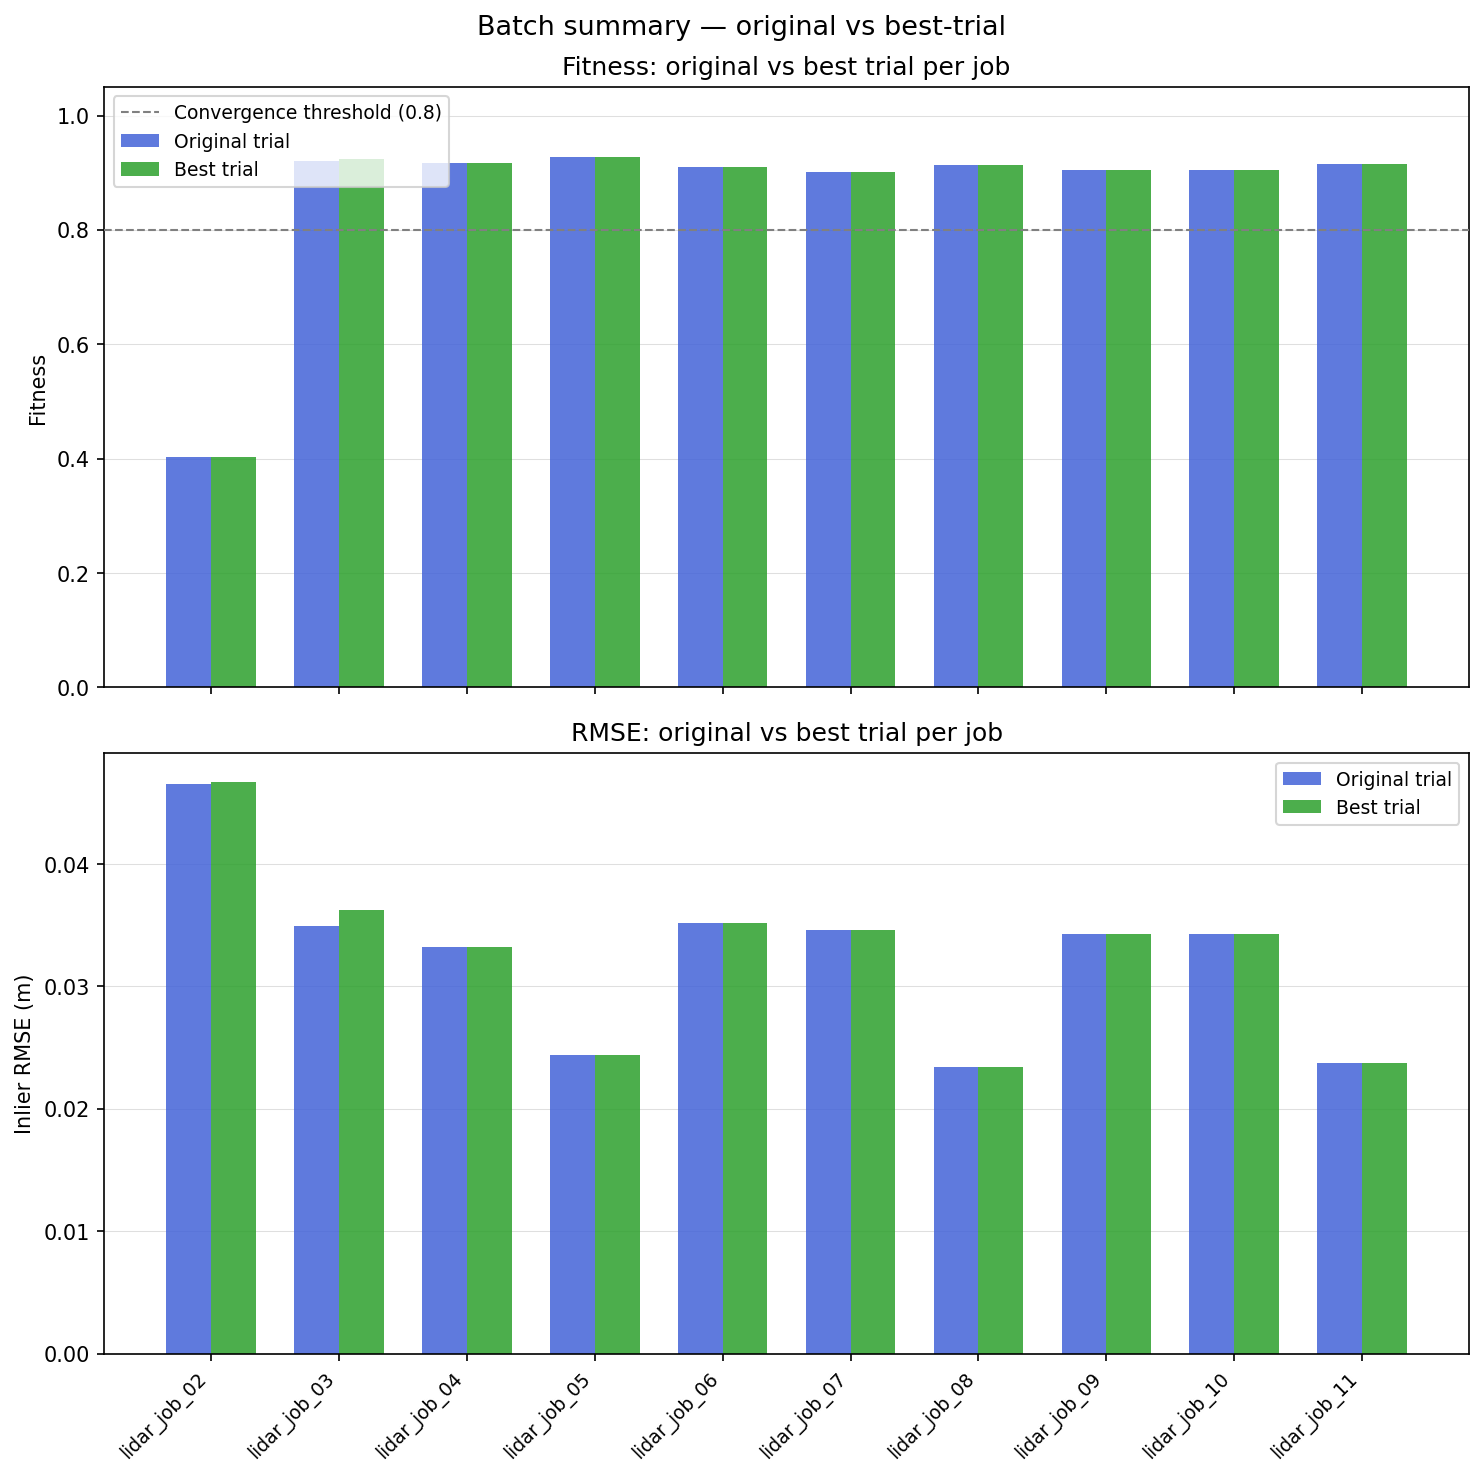
\includegraphics[width=\linewidth]{4-precise-alignment/4-results/figures/lidar_batch_summary}
  \caption{LiDAR batch summary: best-trial fitness and inlier RMSE across all nine conditions. The D110A0 bar visible in this figure was excluded from analysis as it exceeded the stereo pipeline's depth clipping threshold.}
  \label{fig:pa-lidar-batch-summary}
\end{figure}

% ---------------------------------------------------------------------------
\subsection{Stereo Registration Performance}
\label{subsec:pa-results-stereo-summary}
% ---------------------------------------------------------------------------

\Cref{tab:pa-results-stereo-per-condition} summarises the stereo registration outcome for each condition. The stereo pipeline executes a single ICP run per trial; each condition produces exactly one fitness value and one inlier RMSE.

\begin{table}[htbp]
  \centering
  \small
  \setlength{\tabcolsep}{4pt}
  \caption{Per-condition stereo registration summary. Fitness takes a binary value (1.0 or 0.0) because the stereo pipeline executes a single ICP run. Non-converging conditions are listed with dashes for RMSE. All RMSE values in millimetres.}
  \label{tab:pa-results-stereo-per-condition}
  \begin{tabular}{@{} l r r r r r @{}}
    \toprule
    \textbf{Condition} &
    \textbf{Raw pts} &
    \textbf{Proc.\ pts} &
    \boldmath$F$ &
    \boldmath$\varepsilon$ \textbf{(mm)} &
    \textbf{Total time (s)} \\
    \midrule
    D40A$-$15 &  99\,661 & 87\,772 & 1.0 & 16.77 & 14.76 \\
    D40A0     &  97\,181 & 83\,163 & 1.0 & 16.77 & 13.13 \\
    D40A$+$15 &  99\,661 & 87\,994 & 0.0 &  ---  & 11.85 \\
    D60A$-$15 & 107\,944 & 91\,952 & 1.0 & 16.67 & 13.33 \\
    D60A0     &  93\,336 & 68\,811 & 1.0 & 16.76 & 15.08 \\
    D60A$+$15 &  99\,661 & 87\,666 & 1.0 & 16.67 & 12.66 \\
    D80A$-$15 &  81\,464 & 23\,980 & 0.0 &  ---  & 11.82 \\
    D80A0     &  84\,748 & 42\,307 & 1.0 & 12.26 & 20.28 \\
    D80A$+$15 &  81\,464 & 29\,981 & 1.0 & 12.64 & 14.69 \\
    \bottomrule
  \end{tabular}
\end{table}

Seven of nine conditions converged (78\%). Two conditions failed: D40A$+$15 (87\,994 processed points, $F = 0.0$) and D80A$-$15 (23\,980 processed points, $F = 0.0$).

% ---------------------------------------------------------------------------
\subsection{Stereo: Distance and Angle Effects}
\label{subsec:pa-results-stereo-distance-angle}
% ---------------------------------------------------------------------------

\Cref{tab:pa-results-stereo-by-distance,tab:pa-results-stereo-by-angle} present stereo registration outcomes grouped by distance and angle.

\begin{table}[htbp]
  \centering
  \caption{Stereo registration results grouped by sensor-to-vine distance. RMSE computed over converging conditions only. All values in millimetres.}
  \label{tab:pa-results-stereo-by-distance}
  \begin{tabular}{@{} l r r r @{}}
    \toprule
    \textbf{Distance} &
    \textbf{Converged / Total} &
    \textbf{Conv.\ rate (\%)} &
    \textbf{Median} \boldmath$\varepsilon$ \textbf{(mm)} \\
    \midrule
    D40 (40\,cm)   & 2/3 &  67 & 16.77 \\
    D60 (60\,cm)   & 3/3 & 100 & 16.67 \\
    D80 (80\,cm)   & 2/3 &  67 & 12.45 \\
    \bottomrule
  \end{tabular}
\end{table}

\begin{table}[htbp]
  \centering
  \caption{Stereo registration results grouped by approach angle. RMSE computed over converging conditions only. All values in millimetres.}
  \label{tab:pa-results-stereo-by-angle}
  \begin{tabular}{@{} l r r r @{}}
    \toprule
    \textbf{Angle} &
    \textbf{Converged / Total} &
    \textbf{Conv.\ rate (\%)} &
    \textbf{Median} \boldmath$\varepsilon$ \textbf{(mm)} \\
    \midrule
    A$-$15 ($-15^{\circ}$) & 2/3 &  67 & 16.72 \\
    A0 ($0^{\circ}$)       & 3/3 & 100 & 16.76 \\
    A$+$15 ($+15^{\circ}$) & 2/3 &  67 & 14.66 \\
    \bottomrule
  \end{tabular}
\end{table}

D60 achieved full convergence (3/3). The D80 group exhibits lower RMSE (12.45\,mm) compared to D40 (16.77\,mm) and D60 (16.67\,mm). Convergence rates range from 67\% (A$-$15, A$+$15) to 100\% (A0).

% ---------------------------------------------------------------------------
\subsection{Stereo: Recovered ICP Correction}
\label{subsec:pa-results-stereo-transformation}
% ---------------------------------------------------------------------------

\Cref{tab:pa-results-stereo-transforms} reports the positional displacement and rotation correction applied by the GICP solver for each converging condition. The translational displacement $\lVert\Delta\mathbf{t}\rVert$ is the Euclidean distance between the initial and final sensor positions; component displacements ($\Delta x$, $\Delta y$, $\Delta z$) are in the local ENU frame. Rotations are ZYX Euler angles extracted from the correction matrix.

\begin{table}[htbp]
  \centering
  \small
  \setlength{\tabcolsep}{3pt}
  \caption{ICP correction for converging stereo conditions. Translational displacement in millimetres; rotation corrections as ZYX Euler angles in degrees. Non-converging conditions (D80A$-$15, D40A$+$15) omitted.}
  \label{tab:pa-results-stereo-transforms}
  \begin{tabular}{@{} l r r r r r r r @{}}
    \toprule
    \textbf{Condition} &
    \boldmath$\lVert\Delta\mathbf{t}\rVert$ \textbf{(mm)} &
    \boldmath$\Delta x$ \textbf{(mm)} &
    \boldmath$\Delta y$ \textbf{(mm)} &
    \boldmath$\Delta z$ \textbf{(mm)} &
    \boldmath$\Delta\psi$ \textbf{(°)} &
    \boldmath$\Delta\theta$ \textbf{(°)} &
    \boldmath$\Delta\phi$ \textbf{(°)} \\
    \midrule
    D40A$-$15 &  86.3 & $-$17.5 &    76.8 &    35.4 & $-$1.65 &    0.67 & $-$2.46 \\
    D40A0     &  67.5 &    44.4 &    47.8 &    17.2 &    2.25 & $-$1.15 & $-$3.43 \\
    D60A$-$15 & 117.7 & $-$34.6 &   106.3 &    36.9 & $-$3.85 & $-$0.34 & $-$4.15 \\
    D60A0     &  63.7 & $-$23.5 &    48.9 &    33.4 & $-$2.12 & $-$1.48 & $-$3.36 \\
    D60A$+$15 &  46.6 &     8.1 &    35.0 &    29.6 & $-$1.21 &    0.73 & $-$3.08 \\
    D80A0     & 140.6 &  $-$5.2 &    79.9 &   115.6 & $-$0.74 & $-$3.24 & $-$6.60 \\
    D80A$+$15 &  91.4 & $-$22.5 &    63.2 &    62.1 & $-$2.69 & $-$4.49 & $-$3.77 \\
    \bottomrule
  \end{tabular}
\end{table}

For the seven converging conditions, the mean positional displacement is 87.7\,mm (max 140.6\,mm, D80A0), confirming that ICP adjustments remain within the expected range of the initial pose estimate. The roll correction ($\Delta\phi$) is consistently negative, ranging from $-2.5^{\circ}$ to $-6.6^{\circ}$. Rotational corrections are smaller than the LiDAR equivalents, with all angles below $6.6^{\circ}$.

% ---------------------------------------------------------------------------
\subsection{Stereo: Pipeline Timing}
\label{subsec:pa-results-stereo-timing}
% ---------------------------------------------------------------------------

\Cref{tab:pa-results-stereo-timing} reports wall-clock timing for each stereo trial, decomposed into four stages: depth estimation (FoundationStereo inference and back-projection), dual-camera combination, preprocessing (morphological closing, DBSCAN, voxel density filtering), and ICP alignment.

\begin{table}[htbp]
  \centering
  \small
  \setlength{\tabcolsep}{4pt}
  \caption{Per-condition stereo pipeline timing. All values in seconds. No scan accumulation interval precedes the pipeline.}
  \label{tab:pa-results-stereo-timing}
  \begin{tabular}{@{} l r r r r r @{}}
    \toprule
    \textbf{Condition} &
    \textbf{Depth (s)} &
    \textbf{Combine (s)} &
    \textbf{Process (s)} &
    \textbf{ICP (s)} &
    \textbf{Total (s)} \\
    \midrule
    D40A$-$15 & 1.25 & 4.46 & 1.08 &  7.96 & 14.76 \\
    D40A0     & 1.24 & 4.51 & 0.94 &  6.44 & 13.13 \\
    D40A$+$15 & 1.25 & 4.46 & 1.10 &  5.04 & 11.85 \\
    D60A$-$15 & 1.26 & 4.42 & 1.02 &  6.64 & 13.33 \\
    D60A0     & 1.23 & 4.72 & 0.88 &  8.25 & 15.08 \\
    D60A$+$15 & 1.24 & 4.68 & 1.10 &  5.64 & 12.66 \\
    D80A$-$15 & 1.20 & 4.61 & 0.86 &  5.15 & 11.82 \\
    D80A0     & 1.20 & 4.94 & 0.78 & 13.36 & 20.28 \\
    D80A$+$15 & 1.20 & 4.61 & 0.71 &  8.17 & 14.69 \\
    \midrule
    \textbf{Mean $\pm$ std} & $1.23 \pm 0.02$ & $4.60 \pm 0.16$ & $0.94 \pm 0.14$ & $7.41 \pm 2.56$ & $14.18 \pm 2.59$ \\
    \bottomrule
  \end{tabular}
\end{table}

Total pipeline latency ranges from 11.82\,s (D80A$-$15) to 20.28\,s (D80A0), with a mean of $14.18 \pm 2.59$\,s. Depth estimation is consistent at approximately 1.2\,s. The dominant timing components are dual-camera combination ($4.60 \pm 0.16$\,s) and ICP alignment ($7.41 \pm 2.56$\,s).

% ---------------------------------------------------------------------------
\subsection{Stereo: Visual Alignment}
\label{subsec:pa-results-stereo-visual}
% ---------------------------------------------------------------------------

\Cref{fig:pa-stereo-icp-comparison} presents before-and-after ICP alignment comparisons for a representative converging condition (D80A0) and a representative non-converging condition (D40A$+$15).

\begin{figure}[htbp]
  \centering
  \begin{subfigure}[b]{0.48\linewidth}
    \centering
    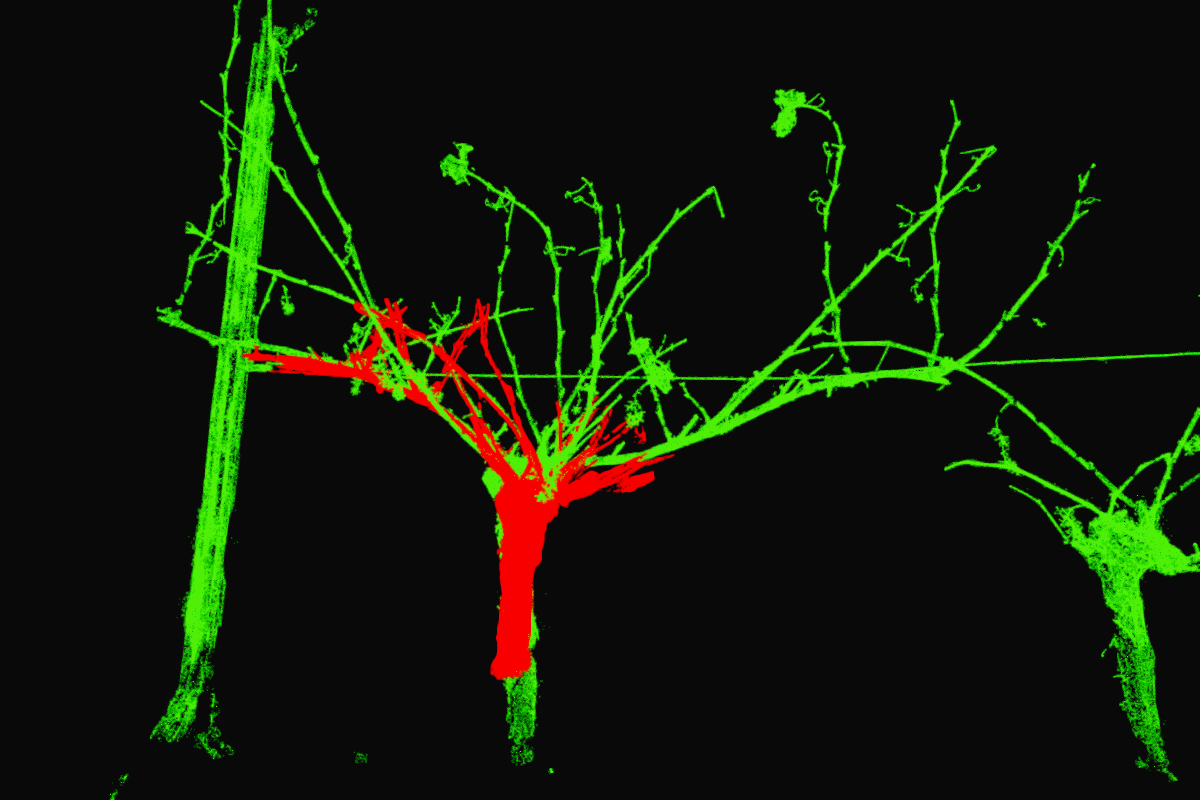
\includegraphics[width=\linewidth]{4-precise-alignment/4-results/figures/stereo_D80A0_4b_icp_initial_side}
    \caption{D80A0: before registration.}
    \label{fig:stereo-D80A0-initial}
  \end{subfigure}
  \hfill
  \begin{subfigure}[b]{0.48\linewidth}
    \centering
    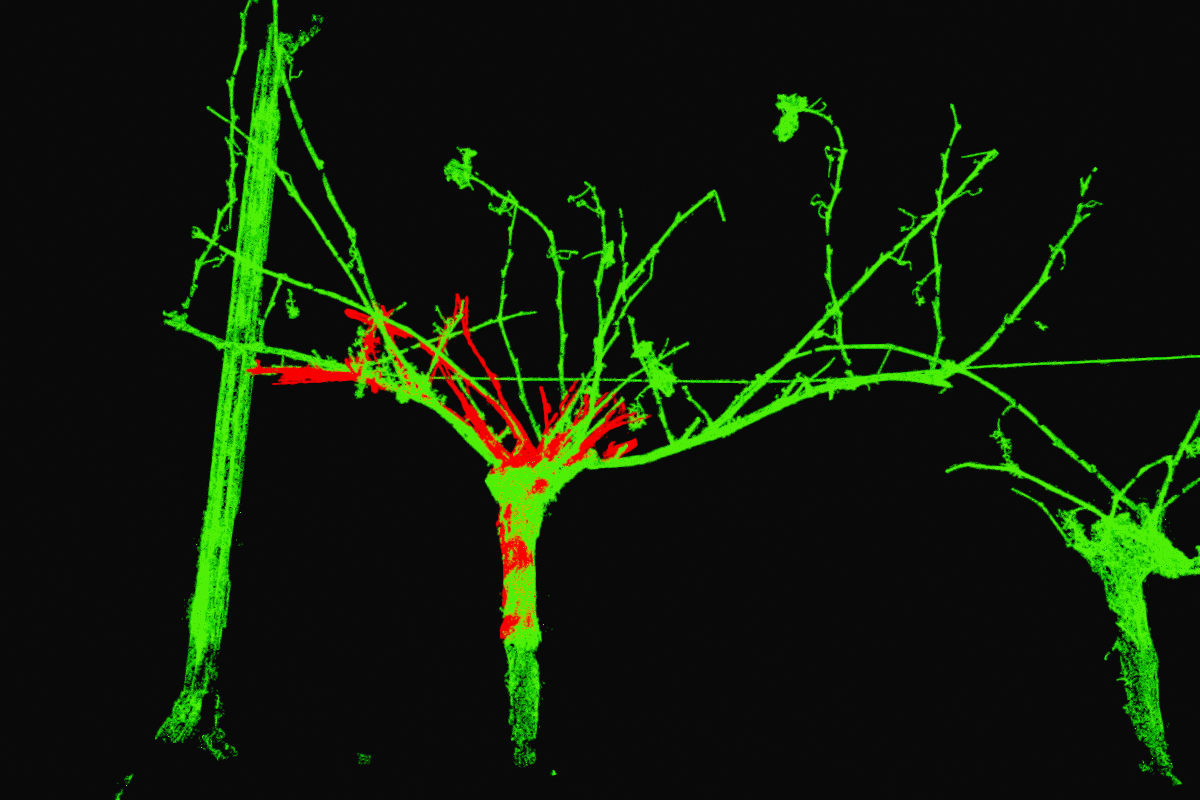
\includegraphics[width=\linewidth]{4-precise-alignment/4-results/figures/stereo_D80A0_5b_icp_final_side}
    \caption{D80A0: after registration ($\varepsilon = 12.26$\,mm).}
    \label{fig:stereo-D80A0-final}
  \end{subfigure}

  \vspace{0.5em}

  \begin{subfigure}[b]{0.48\linewidth}
    \centering
    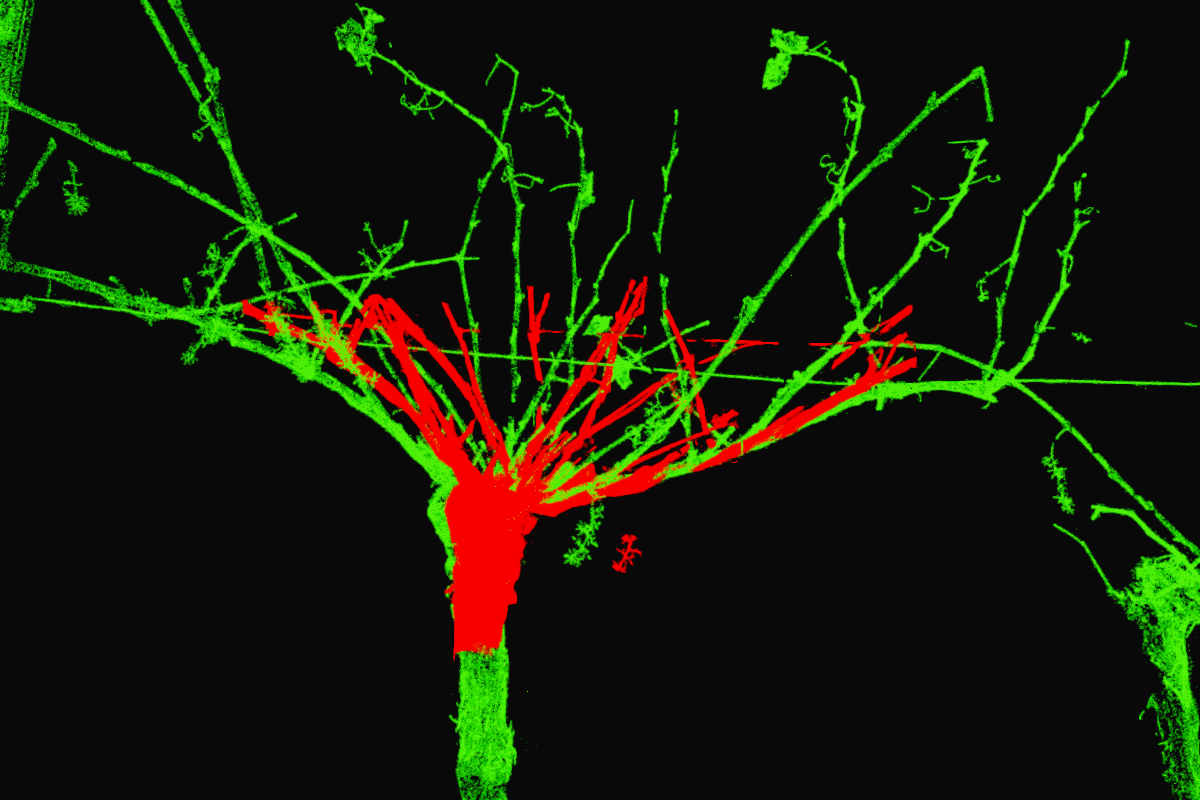
\includegraphics[width=\linewidth]{4-precise-alignment/4-results/figures/stereo_D40Ap15_4b_icp_initial_side}
    \caption{D40A$+$15: before registration.}
    \label{fig:stereo-D40Ap15-initial}
  \end{subfigure}
  \hfill
  \begin{subfigure}[b]{0.48\linewidth}
    \centering
    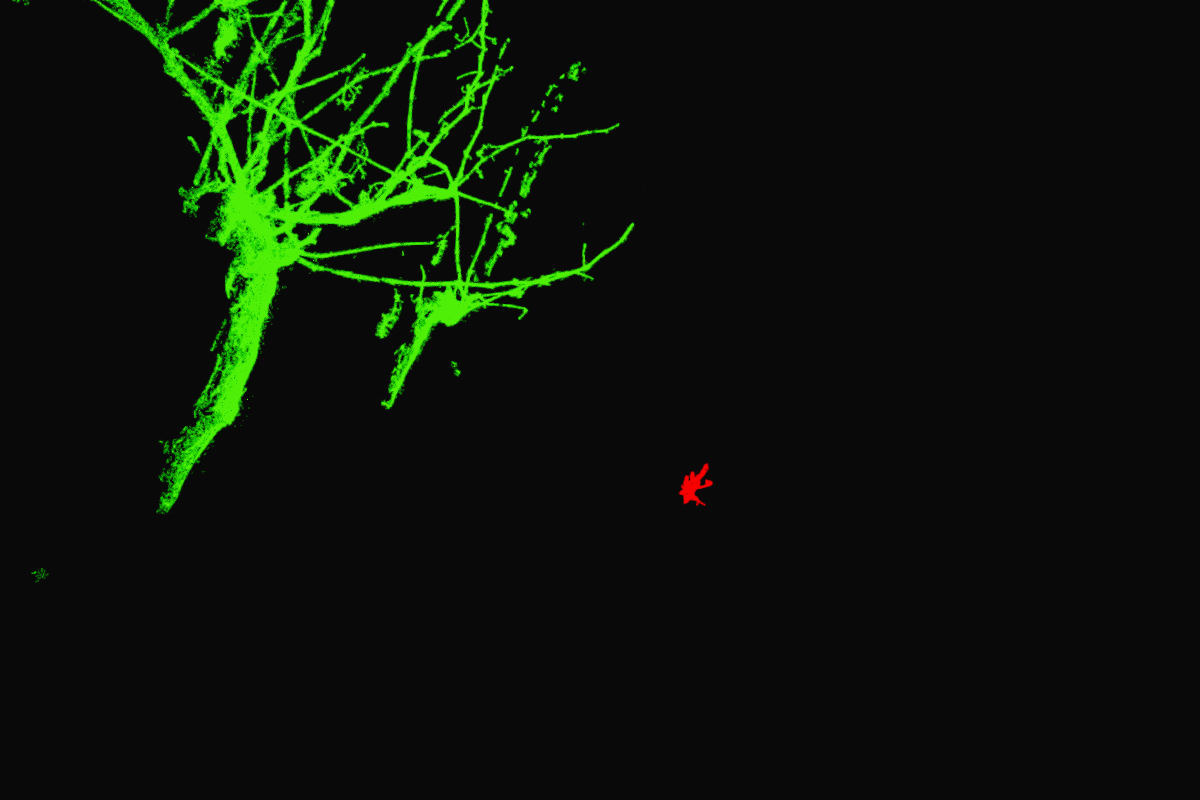
\includegraphics[width=\linewidth]{4-precise-alignment/4-results/figures/stereo_D40Ap15_5b_icp_final_side}
    \caption{D40A$+$15: after registration (failed, $F = 0.0$).}
    \label{fig:stereo-D40Ap15-final}
  \end{subfigure}
  \caption{Stereo ICP alignment comparison (vine-face view). Top row: D80A0, a converging trial achieving 12.26\,mm RMSE. Bottom row: D40A$+$15, a non-converging trial. Green: 3DGS reference cloud; red: stereo source cloud.}
  \label{fig:pa-stereo-icp-comparison}
\end{figure}

\Cref{fig:pa-stereo-converged-overlay} presents the final alignment for all seven converging conditions.

\begin{figure}[htbp]
  \centering
  \begin{subfigure}[b]{0.32\linewidth}
    \centering
    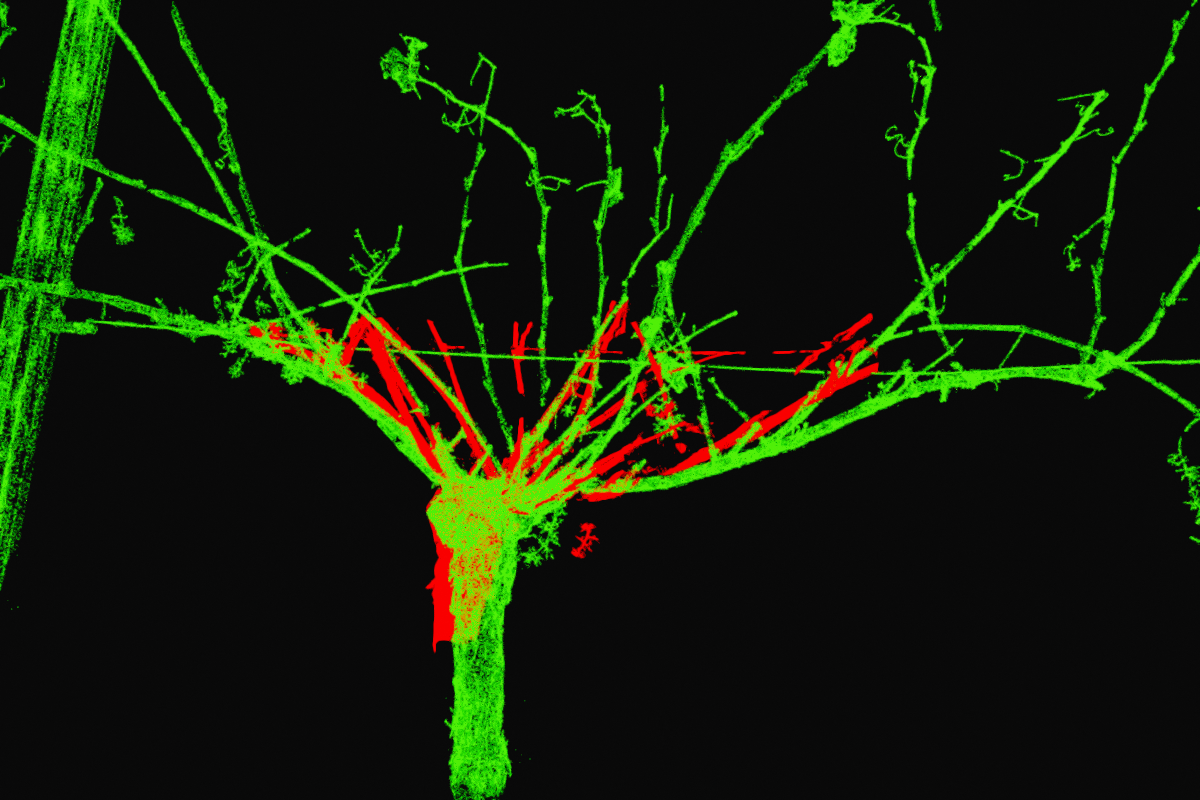
\includegraphics[width=\linewidth]{4-precise-alignment/4-results/figures/stereo_D40Am15_5b_icp_final_side}
    \caption{D40A$-$15}
  \end{subfigure}
  \hfill
  \begin{subfigure}[b]{0.32\linewidth}
    \centering
    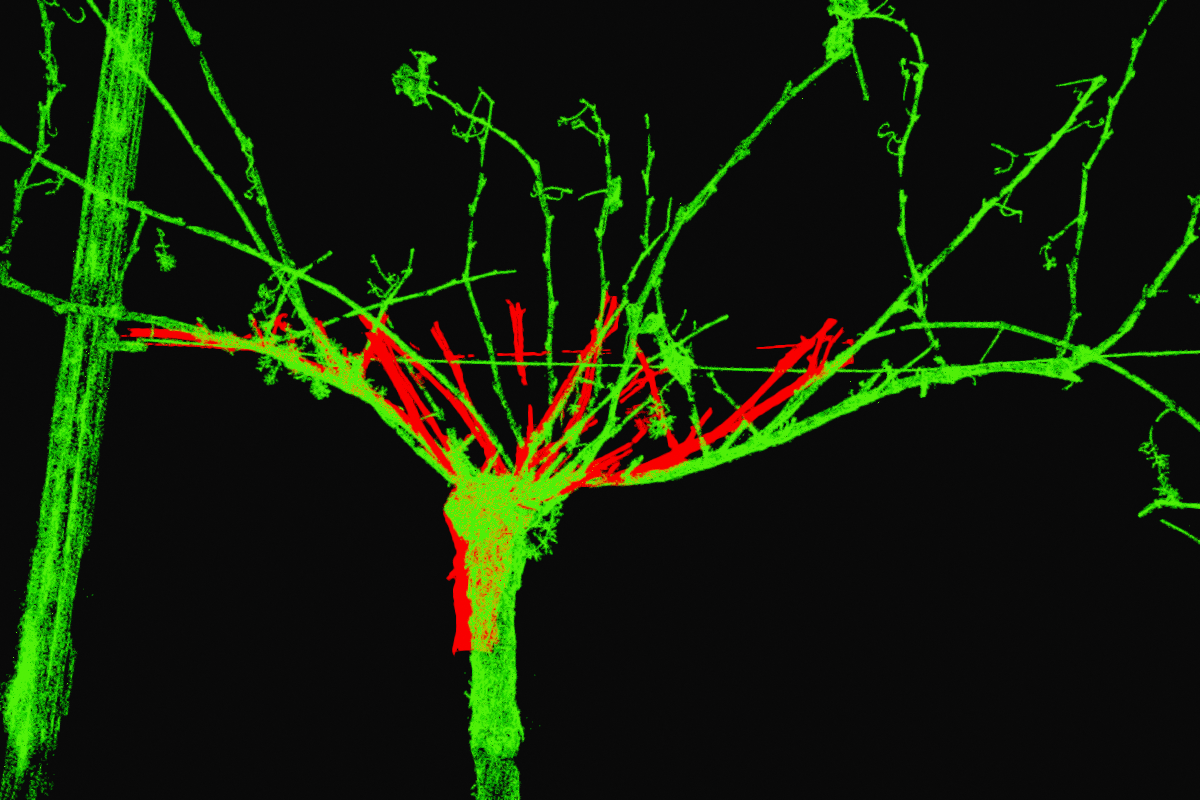
\includegraphics[width=\linewidth]{4-precise-alignment/4-results/figures/stereo_D40A0_5b_icp_final_side}
    \caption{D40A0}
  \end{subfigure}
  \hfill
  \begin{subfigure}[b]{0.32\linewidth}
    \centering
    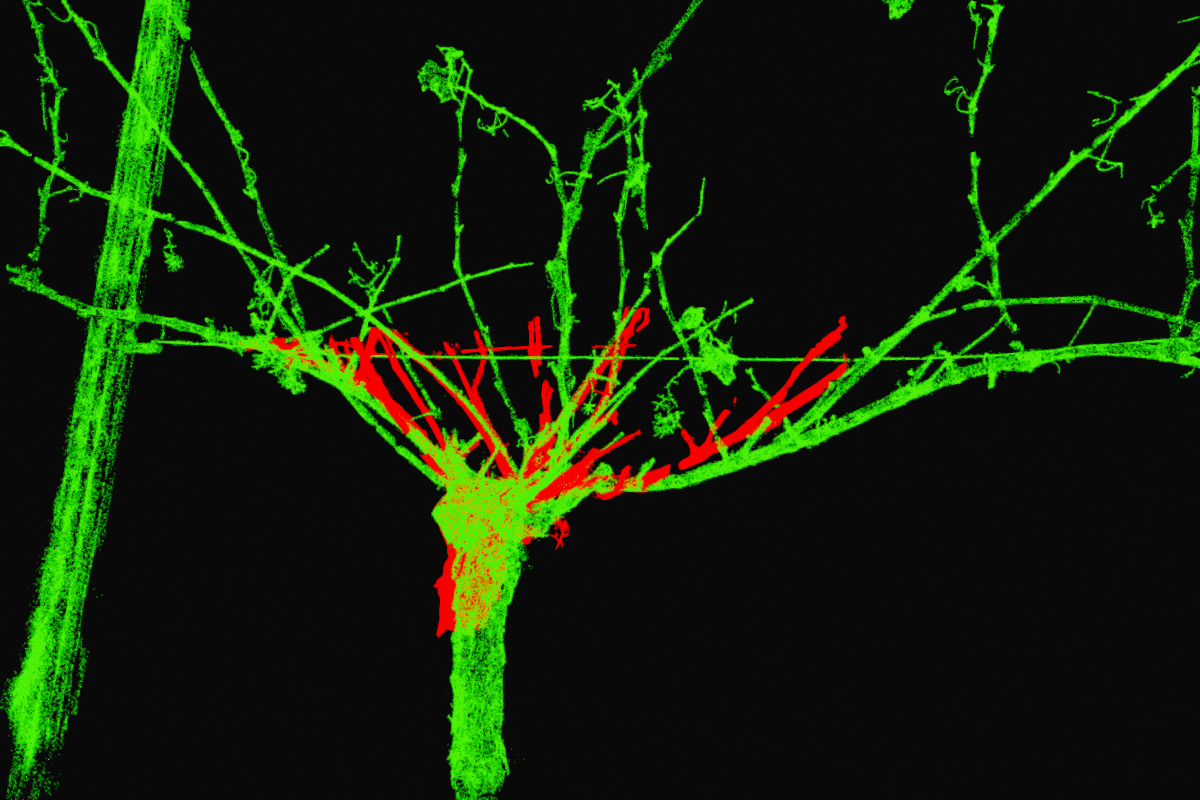
\includegraphics[width=\linewidth]{4-precise-alignment/4-results/figures/stereo_D60Am15_5b_icp_final_side}
    \caption{D60A$-$15}
  \end{subfigure}

  \vspace{0.5em}

  \begin{subfigure}[b]{0.32\linewidth}
    \centering
    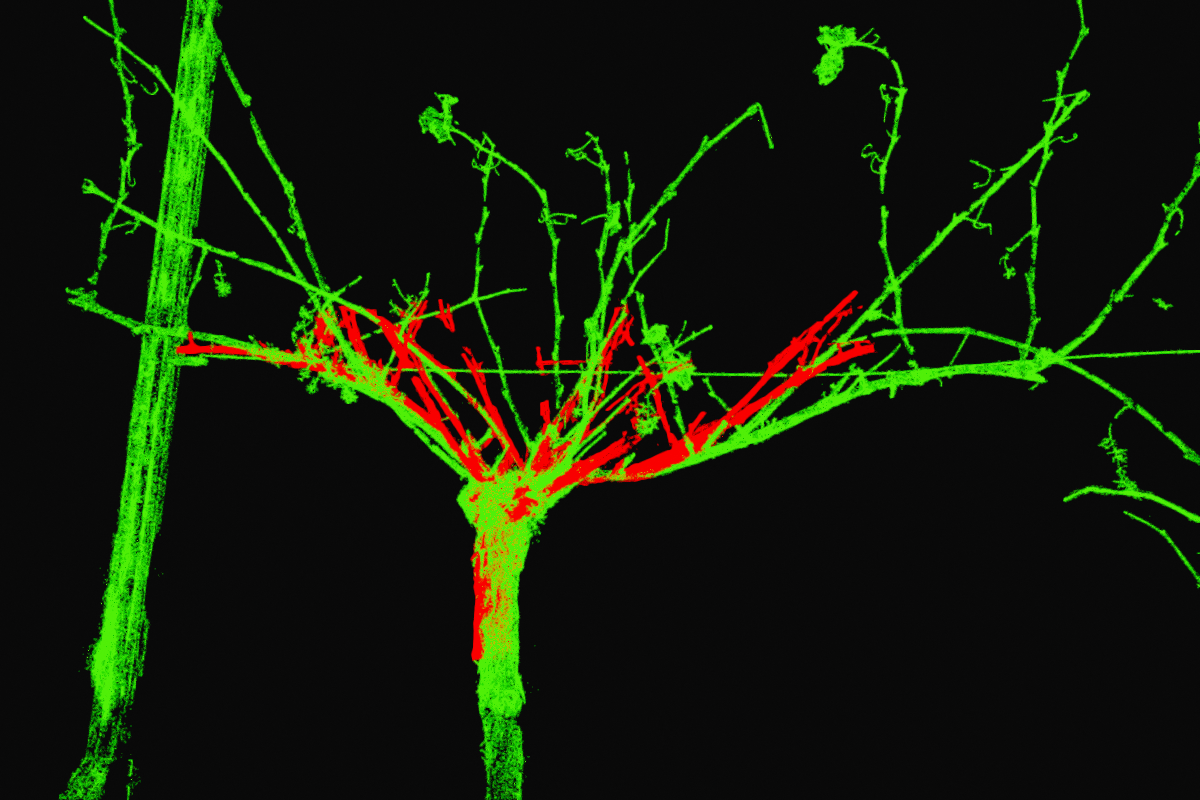
\includegraphics[width=\linewidth]{4-precise-alignment/4-results/figures/stereo_D60A0_5b_icp_final_side}
    \caption{D60A0}
  \end{subfigure}
  \hfill
  \begin{subfigure}[b]{0.32\linewidth}
    \centering
    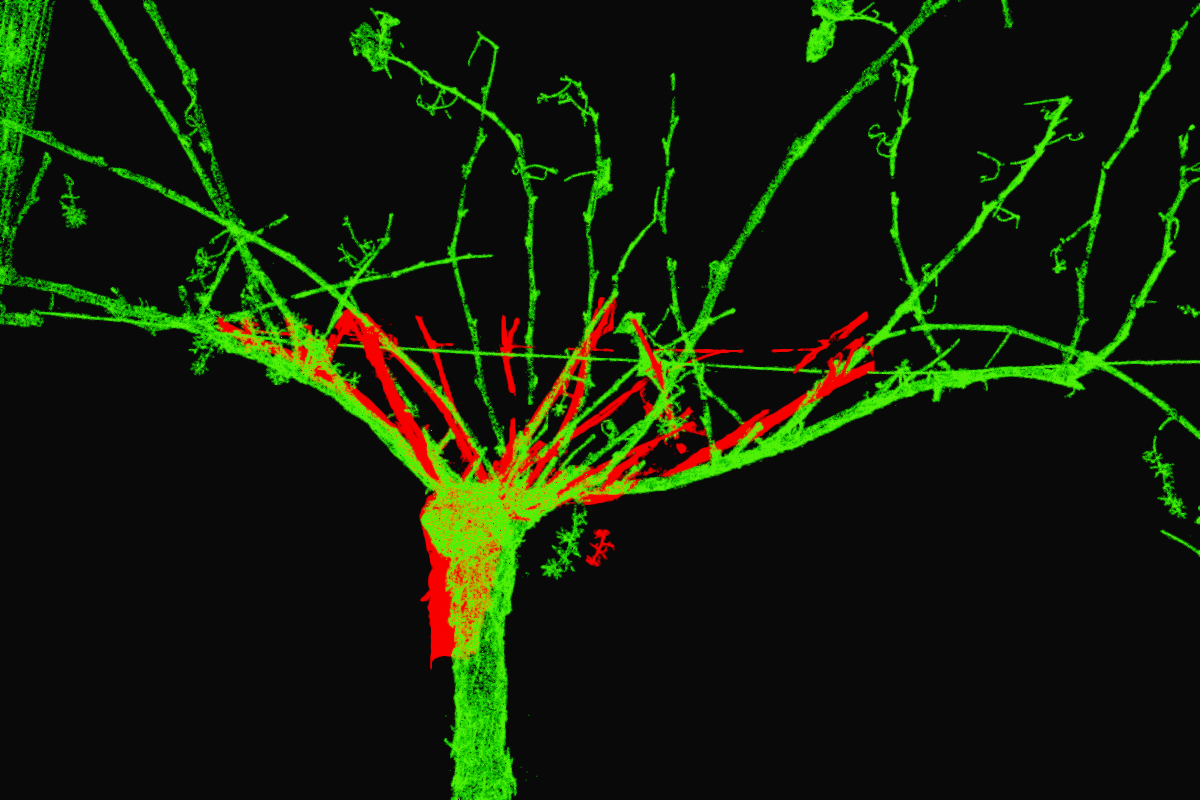
\includegraphics[width=\linewidth]{4-precise-alignment/4-results/figures/stereo_D60Ap15_5b_icp_final_side}
    \caption{D60A$+$15}
  \end{subfigure}
  \hfill
  \begin{subfigure}[b]{0.32\linewidth}
    \centering
    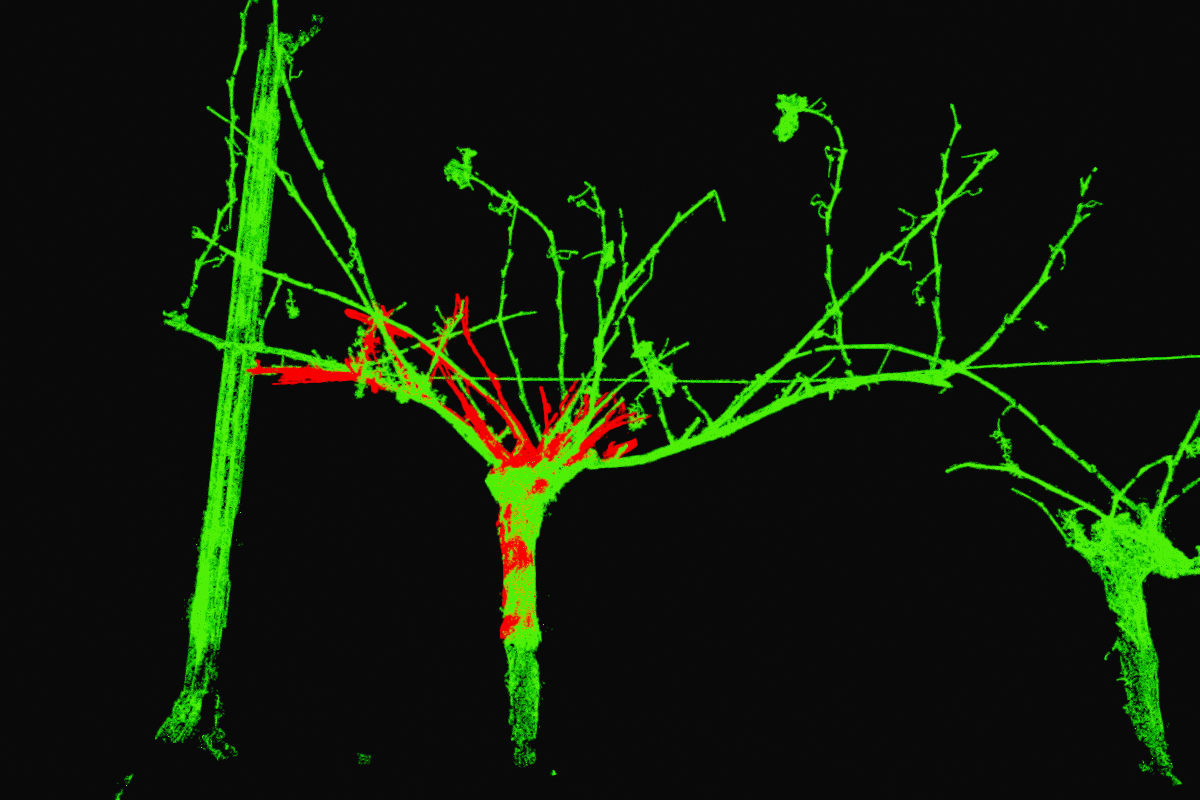
\includegraphics[width=\linewidth]{4-precise-alignment/4-results/figures/stereo_D80A0_5b_icp_final_side}
    \caption{D80A0}
  \end{subfigure}

  \vspace{0.5em}

  \begin{subfigure}[b]{0.32\linewidth}
    \centering
    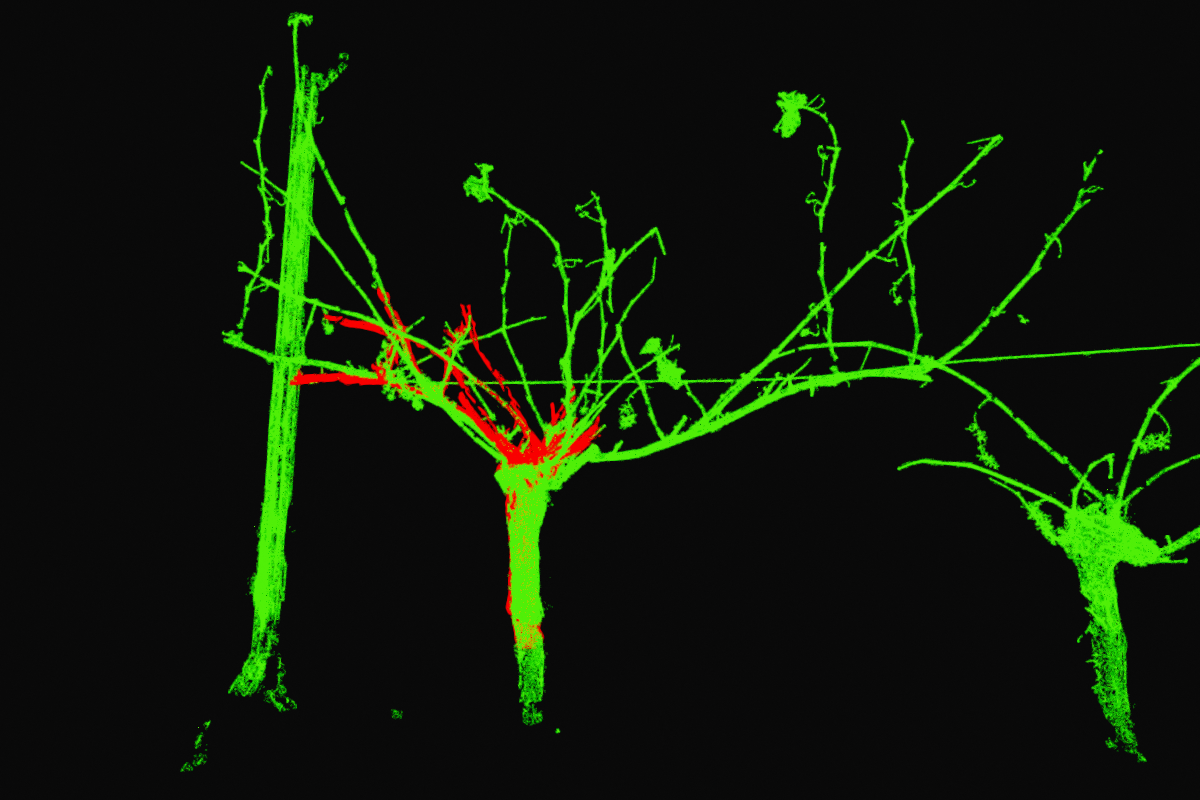
\includegraphics[width=\linewidth]{4-precise-alignment/4-results/figures/stereo_D80Ap15_5b_icp_final_side}
    \caption{D80A$+$15}
  \end{subfigure}
  \caption{Final stereo ICP alignment (vine-face view) for all seven converging conditions. Green: 3DGS reference cloud; red: registered stereo source cloud.}
  \label{fig:pa-stereo-converged-overlay}
\end{figure}

% ---------------------------------------------------------------------------
\subsection{Cross-Modal Comparison}
\label{subsec:pa-results-cross-modal}
% ---------------------------------------------------------------------------

\Cref{tab:pa-results-cross-modal} presents a matched-condition comparison of LiDAR and stereo registration outcomes. Each row corresponds to one experimental condition.

\begin{table}[htbp]
  \centering
  \small
  \setlength{\tabcolsep}{4pt}
  \caption{Matched-condition comparison of LiDAR and stereo registration outcomes. LiDAR $n_\text{acc}$: accepted hypotheses out of 35; $\tilde{\varepsilon}$: median inlier RMSE across accepted hypotheses. Stereo $\varepsilon$: single-run inlier RMSE for converging conditions. All RMSE values in millimetres.}
  \label{tab:pa-results-cross-modal}
  \begin{tabular}{@{} l r r c r @{}}
    \toprule
    \textbf{Condition} &
    \textbf{LiDAR} \boldmath$n_\text{acc}$\textbf{/35} &
    \textbf{LiDAR} \boldmath$\tilde{\varepsilon}$ \textbf{(mm)} &
    \textbf{Stereo conv.} &
    \textbf{Stereo} \boldmath$\varepsilon$ \textbf{(mm)} \\
    \midrule
    D40A$-$15 & 35/35 & 32.31 & Yes & 16.77 \\
    D40A0     & 34/35 & 35.22 & Yes & 16.77 \\
    D40A$+$15 & 35/35 & 34.85 & No  &  ---  \\
    D60A$-$15 & 35/35 & 34.94 & Yes & 16.67 \\
    D60A0     & 35/35 & 33.25 & Yes & 16.76 \\
    D60A$+$15 & 35/35 & 34.84 & Yes & 16.67 \\
    D80A$-$15 & 35/35 & 23.38 & No  &  ---  \\
    D80A0     & 32/35 & 24.41 & Yes & 12.26 \\
    D80A$+$15 & 35/35 & 23.77 & Yes & 12.64 \\
    \midrule
    \textbf{Both converged (mean)} & --- & 31.40 & --- & 15.51 \\
    \bottomrule
  \end{tabular}
\end{table}

LiDAR achieved convergence ($\geq 1$ accepted hypothesis) in all 9 conditions (100\%); stereo converged in 7 of 9 (78\%). On the seven conditions where both pipelines converged, the mean stereo RMSE is 15.51\,mm versus 31.40\,mm for LiDAR. LiDAR converged in two conditions where stereo failed (D40A$+$15 and D80A$-$15); no condition that failed for LiDAR succeeded for stereo. The mean stereo pipeline latency across all conditions is $14.18 \pm 2.59$\,s, compared to $46.0 \pm 3.8$\,s for LiDAR (excluding the 25\,s accumulation interval).
